% Options for packages loaded elsewhere
\PassOptionsToPackage{unicode}{hyperref}
\PassOptionsToPackage{hyphens}{url}
%
\documentclass[
  18 pt,
  ignorenonframetext,
  aspectratio=1610,
]{beamer}
\usepackage{pgfpages}
\setbeamertemplate{caption}[numbered]
\setbeamertemplate{caption label separator}{: }
\setbeamercolor{caption name}{fg=normal text.fg}
\beamertemplatenavigationsymbolshorizontal
% Prevent slide breaks in the middle of a paragraph
\widowpenalties 1 10000
\raggedbottom
\setbeamertemplate{part page}{
  \centering
  \begin{beamercolorbox}[sep=16pt,center]{part title}
    \usebeamerfont{part title}\insertpart\par
  \end{beamercolorbox}
}
\setbeamertemplate{section page}{
  \centering
  \begin{beamercolorbox}[sep=12pt,center]{part title}
    \usebeamerfont{section title}\insertsection\par
  \end{beamercolorbox}
}
\setbeamertemplate{subsection page}{
  \centering
  \begin{beamercolorbox}[sep=8pt,center]{part title}
    \usebeamerfont{subsection title}\insertsubsection\par
  \end{beamercolorbox}
}
\AtBeginPart{
  \frame{\partpage}
}
\AtBeginSection{
  \ifbibliography
  \else
    \frame{\sectionpage}
  \fi
}
\AtBeginSubsection{
  \frame{\subsectionpage}
}

\usepackage{amsmath,amssymb}
\usepackage{iftex}
\ifPDFTeX
  \usepackage[T1]{fontenc}
  \usepackage[utf8]{inputenc}
  \usepackage{textcomp} % provide euro and other symbols
\else % if luatex or xetex
  \usepackage{unicode-math}
  \defaultfontfeatures{Scale=MatchLowercase}
  \defaultfontfeatures[\rmfamily]{Ligatures=TeX,Scale=1}
\fi
\usepackage{lmodern}
\usetheme[]{AnnArbor}
\usecolortheme{dolphin}
\usefonttheme{structurebold}
\ifPDFTeX\else  
    % xetex/luatex font selection
\fi
% Use upquote if available, for straight quotes in verbatim environments
\IfFileExists{upquote.sty}{\usepackage{upquote}}{}
\IfFileExists{microtype.sty}{% use microtype if available
  \usepackage[]{microtype}
  \UseMicrotypeSet[protrusion]{basicmath} % disable protrusion for tt fonts
}{}
\makeatletter
\@ifundefined{KOMAClassName}{% if non-KOMA class
  \IfFileExists{parskip.sty}{%
    \usepackage{parskip}
  }{% else
    \setlength{\parindent}{0pt}
    \setlength{\parskip}{6pt plus 2pt minus 1pt}}
}{% if KOMA class
  \KOMAoptions{parskip=half}}
\makeatother
\usepackage{xcolor}
\newif\ifbibliography
\setlength{\emergencystretch}{3em} % prevent overfull lines
\setcounter{secnumdepth}{-\maxdimen} % remove section numbering

\usepackage{color}
\usepackage{fancyvrb}
\newcommand{\VerbBar}{|}
\newcommand{\VERB}{\Verb[commandchars=\\\{\}]}
\DefineVerbatimEnvironment{Highlighting}{Verbatim}{commandchars=\\\{\}}
% Add ',fontsize=\small' for more characters per line
\usepackage{framed}
\definecolor{shadecolor}{RGB}{241,243,245}
\newenvironment{Shaded}{\begin{snugshade}}{\end{snugshade}}
\newcommand{\AlertTok}[1]{\textcolor[rgb]{0.68,0.00,0.00}{#1}}
\newcommand{\AnnotationTok}[1]{\textcolor[rgb]{0.37,0.37,0.37}{#1}}
\newcommand{\AttributeTok}[1]{\textcolor[rgb]{0.40,0.45,0.13}{#1}}
\newcommand{\BaseNTok}[1]{\textcolor[rgb]{0.68,0.00,0.00}{#1}}
\newcommand{\BuiltInTok}[1]{\textcolor[rgb]{0.00,0.23,0.31}{#1}}
\newcommand{\CharTok}[1]{\textcolor[rgb]{0.13,0.47,0.30}{#1}}
\newcommand{\CommentTok}[1]{\textcolor[rgb]{0.37,0.37,0.37}{#1}}
\newcommand{\CommentVarTok}[1]{\textcolor[rgb]{0.37,0.37,0.37}{\textit{#1}}}
\newcommand{\ConstantTok}[1]{\textcolor[rgb]{0.56,0.35,0.01}{#1}}
\newcommand{\ControlFlowTok}[1]{\textcolor[rgb]{0.00,0.23,0.31}{#1}}
\newcommand{\DataTypeTok}[1]{\textcolor[rgb]{0.68,0.00,0.00}{#1}}
\newcommand{\DecValTok}[1]{\textcolor[rgb]{0.68,0.00,0.00}{#1}}
\newcommand{\DocumentationTok}[1]{\textcolor[rgb]{0.37,0.37,0.37}{\textit{#1}}}
\newcommand{\ErrorTok}[1]{\textcolor[rgb]{0.68,0.00,0.00}{#1}}
\newcommand{\ExtensionTok}[1]{\textcolor[rgb]{0.00,0.23,0.31}{#1}}
\newcommand{\FloatTok}[1]{\textcolor[rgb]{0.68,0.00,0.00}{#1}}
\newcommand{\FunctionTok}[1]{\textcolor[rgb]{0.28,0.35,0.67}{#1}}
\newcommand{\ImportTok}[1]{\textcolor[rgb]{0.00,0.46,0.62}{#1}}
\newcommand{\InformationTok}[1]{\textcolor[rgb]{0.37,0.37,0.37}{#1}}
\newcommand{\KeywordTok}[1]{\textcolor[rgb]{0.00,0.23,0.31}{#1}}
\newcommand{\NormalTok}[1]{\textcolor[rgb]{0.00,0.23,0.31}{#1}}
\newcommand{\OperatorTok}[1]{\textcolor[rgb]{0.37,0.37,0.37}{#1}}
\newcommand{\OtherTok}[1]{\textcolor[rgb]{0.00,0.23,0.31}{#1}}
\newcommand{\PreprocessorTok}[1]{\textcolor[rgb]{0.68,0.00,0.00}{#1}}
\newcommand{\RegionMarkerTok}[1]{\textcolor[rgb]{0.00,0.23,0.31}{#1}}
\newcommand{\SpecialCharTok}[1]{\textcolor[rgb]{0.37,0.37,0.37}{#1}}
\newcommand{\SpecialStringTok}[1]{\textcolor[rgb]{0.13,0.47,0.30}{#1}}
\newcommand{\StringTok}[1]{\textcolor[rgb]{0.13,0.47,0.30}{#1}}
\newcommand{\VariableTok}[1]{\textcolor[rgb]{0.07,0.07,0.07}{#1}}
\newcommand{\VerbatimStringTok}[1]{\textcolor[rgb]{0.13,0.47,0.30}{#1}}
\newcommand{\WarningTok}[1]{\textcolor[rgb]{0.37,0.37,0.37}{\textit{#1}}}

\providecommand{\tightlist}{%
  \setlength{\itemsep}{0pt}\setlength{\parskip}{0pt}}\usepackage{longtable,booktabs,array}
\usepackage{calc} % for calculating minipage widths
\usepackage{caption}
% Make caption package work with longtable
\makeatletter
\def\fnum@table{\tablename~\thetable}
\makeatother
\usepackage{graphicx}
\makeatletter
\def\maxwidth{\ifdim\Gin@nat@width>\linewidth\linewidth\else\Gin@nat@width\fi}
\def\maxheight{\ifdim\Gin@nat@height>\textheight\textheight\else\Gin@nat@height\fi}
\makeatother
% Scale images if necessary, so that they will not overflow the page
% margins by default, and it is still possible to overwrite the defaults
% using explicit options in \includegraphics[width, height, ...]{}
\setkeys{Gin}{width=\maxwidth,height=\maxheight,keepaspectratio}
% Set default figure placement to htbp
\makeatletter
\def\fps@figure{htbp}
\makeatother

\makeatletter
\makeatother
\makeatletter
\makeatother
\makeatletter
\@ifpackageloaded{caption}{}{\usepackage{caption}}
\AtBeginDocument{%
\ifdefined\contentsname
  \renewcommand*\contentsname{Table of contents}
\else
  \newcommand\contentsname{Table of contents}
\fi
\ifdefined\listfigurename
  \renewcommand*\listfigurename{List of Figures}
\else
  \newcommand\listfigurename{List of Figures}
\fi
\ifdefined\listtablename
  \renewcommand*\listtablename{List of Tables}
\else
  \newcommand\listtablename{List of Tables}
\fi
\ifdefined\figurename
  \renewcommand*\figurename{Figure}
\else
  \newcommand\figurename{Figure}
\fi
\ifdefined\tablename
  \renewcommand*\tablename{Table}
\else
  \newcommand\tablename{Table}
\fi
}
\@ifpackageloaded{float}{}{\usepackage{float}}
\floatstyle{ruled}
\@ifundefined{c@chapter}{\newfloat{codelisting}{h}{lop}}{\newfloat{codelisting}{h}{lop}[chapter]}
\floatname{codelisting}{Listing}
\newcommand*\listoflistings{\listof{codelisting}{List of Listings}}
\makeatother
\makeatletter
\@ifpackageloaded{caption}{}{\usepackage{caption}}
\@ifpackageloaded{subcaption}{}{\usepackage{subcaption}}
\makeatother
\makeatletter
\@ifpackageloaded{tcolorbox}{}{\usepackage[skins,breakable]{tcolorbox}}
\makeatother
\makeatletter
\@ifundefined{shadecolor}{\definecolor{shadecolor}{rgb}{.97, .97, .97}}
\makeatother
\makeatletter
\makeatother
\makeatletter
\makeatother
\ifLuaTeX
  \usepackage{selnolig}  % disable illegal ligatures
\fi
\IfFileExists{bookmark.sty}{\usepackage{bookmark}}{\usepackage{hyperref}}
\IfFileExists{xurl.sty}{\usepackage{xurl}}{} % add URL line breaks if available
\urlstyle{same} % disable monospaced font for URLs
\hypersetup{
  pdftitle={R Programming - Regression},
  pdfauthor={Mahesh Divakaran},
  hidelinks,
  pdfcreator={LaTeX via pandoc}}

\title{R Programming - Regression}
\author{Mahesh Divakaran}
\date{2024-10-07}
\institute{Amity University, Lucknow}
\titlegraphic{
\includegraphics{amity.png}}

\begin{document}
\frame{\titlepage}
\ifdefined\Shaded\renewenvironment{Shaded}{\begin{tcolorbox}[boxrule=0pt, frame hidden, breakable, interior hidden, enhanced, borderline west={3pt}{0pt}{shadecolor}, sharp corners]}{\end{tcolorbox}}\fi

\begin{frame}{Overview}
\protect\hypertarget{overview}{}
\begin{itemize}
\tightlist
\item
  What is Regression
\item
  Mtcars Dataset
\item
  Data exploration (EDA)
\item
  Visualizations
\item
  Simple Linear Regression
\item
  Multiple Linear Regression
\item
  Logistic Regression
\item
  Odds Ratio Interpretation
\end{itemize}
\end{frame}

\hypertarget{what-is-regression}{%
\section{What is Regression?}\label{what-is-regression}}

\begin{frame}{Definition and Purpose}
\protect\hypertarget{definition-and-purpose}{}
\begin{itemize}
\tightlist
\item
  \textbf{Regression} is a statistical technique used to estimate the
  relationships between a dependent variable (response) and one or more
  independent variables (predictors).
\item
  \textbf{Purpose}:

  \begin{itemize}
  \tightlist
  \item
    To understand the strength and direction of the relationship between
    variables.
  \item
    To predict future outcomes based on the relationships observed.
  \end{itemize}
\item
  \textbf{Application}:

  \begin{itemize}
  \tightlist
  \item
    Widely used in fields like medicine, economics, engineering, and the
    social sciences for tasks like forecasting, risk assessment, and
    optimization.
  \end{itemize}
\item
  \textbf{Key Concepts}:

  \begin{itemize}
  \tightlist
  \item
    \textbf{Dependent Variable (Y)}: The outcome you're trying to
    predict or explain.
  \item
    \textbf{Independent Variables (X)}: The predictors used to explain
    or influence Y.
  \item
    \textbf{Error Term (}\(\epsilon\)): Represents the unexplained
    variability in Y.
  \end{itemize}
\end{itemize}
\end{frame}

\begin{frame}{Types of Regression: Linear and Non-Linear Regression}
\protect\hypertarget{types-of-regression-linear-and-non-linear-regression}{}
Regression can be broadly classified into two categories:

\begin{itemize}
\tightlist
\item
  \textbf{Linear Regression}: Models a straight-line relationship
  between the dependent and independent variables.
\item
  \textbf{Non-Linear Regression}: Models a more complex, non-linear
  relationship between variables.
\end{itemize}
\end{frame}

\begin{frame}{Types of Linear Regression}
\protect\hypertarget{types-of-linear-regression}{}
\begin{itemize}
\tightlist
\item
  \textbf{Linear Regression} assumes that the relationship between the
  dependent and independent variables is a straight line. Key types
  include:
\end{itemize}

\scriptsize

\begin{block}{1. Simple Linear Regression}
\protect\hypertarget{simple-linear-regression}{}
\begin{itemize}
\tightlist
\item
  \textbf{Definition}: Models the relationship between one independent
  variable (X) and one dependent variable (Y).
\item
  \textbf{Formula}: \(Y = \beta_0 + \beta_1 X + \epsilon\)
\item
  \textbf{Application}: Predicting outcomes based on a single predictor
  (e.g., predicting salary based on years of experience).
\end{itemize}
\end{block}

\begin{block}{2. Multiple Linear Regression}
\protect\hypertarget{multiple-linear-regression}{}
\begin{itemize}
\tightlist
\item
  \textbf{Definition}: Models the relationship between two or more
  independent variables and a dependent variable.
\item
  \textbf{Formula}:
  \(Y = \beta_0 + \beta_1 X_1 + \beta_2 X_2 + \ldots + \beta_n X_n + \epsilon\)
\item
  \textbf{Application}: Predicting outcomes based on multiple predictors
  (e.g., predicting house prices based on size, location, and number of
  rooms).
\end{itemize}

\normalsize
\end{block}
\end{frame}

\begin{frame}{Types of Non-Linear Regression}
\protect\hypertarget{types-of-non-linear-regression}{}
\scriptsize

\begin{itemize}
\tightlist
\item
  \textbf{Non-Linear Regression} models relationships that cannot be
  captured by a straight line. It is used when the relationship between
  variables is more complex. Key types include:
\end{itemize}

\begin{block}{1. Logistic Regression}
\protect\hypertarget{logistic-regression}{}
\begin{itemize}
\tightlist
\item
  \textbf{Definition}: Used when the dependent variable is binary (0/1
  or Yes/No).
\item
  \textbf{Formula}:
  \(log(p / (1-p)) = \beta_0 + \beta_1X1 + ... + \beta_nXn\)
\item
  \textbf{Application}: Predicting probabilities, such as the likelihood
  of disease presence (yes/no).
\end{itemize}
\end{block}

\begin{block}{2. Poisson Regression}
\protect\hypertarget{poisson-regression}{}
\begin{itemize}
\tightlist
\item
  \textbf{Definition}: Used when the dependent variable represents count
  data (number of occurrences).
\item
  \textbf{Formula}: \(log(λ) = \beta_0 + \beta_1X1 + ... + \beta_nXn\)
\item
  \textbf{Application}: Modeling the number of events, such as customer
  complaints or number of accidents.
\end{itemize}
\end{block}

\begin{block}{3. Polynomial Regression}
\protect\hypertarget{polynomial-regression}{}
\begin{itemize}
\tightlist
\item
  \textbf{Definition}: A form of regression that models the relationship
  as an nth-degree polynomial.
\item
  \textbf{Formula}:
  \(Y = \beta_0 + \beta_1X + \beta_2X^2 + ... + \beta_nX^n + \epsilon\)
\item
  \textbf{Application}: Capturing non-linear trends (e.g., modeling the
  growth curve of a population over time).
\end{itemize}

\normalsize
\end{block}
\end{frame}

\hypertarget{introduction-to-the-mtcars-dataset}{%
\section{Introduction to the mtcars
Dataset}\label{introduction-to-the-mtcars-dataset}}

\begin{frame}{Overview of mtcars}
\protect\hypertarget{overview-of-mtcars}{}
\begin{itemize}
\tightlist
\item
  The \textbf{mtcars} dataset is built into R and contains data about
  various models of cars from the 1974 Motor Trend US magazine. - It
  includes 32 observations (cars) and 11 variables (attributes).
\end{itemize}

\begin{block}{Variables in the mtcars Dataset}
\protect\hypertarget{variables-in-the-mtcars-dataset}{}
\begin{itemize}
\tightlist
\item
  \textbf{mpg}: Miles per gallon (fuel efficiency)
\item
  \textbf{cyl}: Number of cylinders in the car
\item
  \textbf{disp}: Displacement (in cubic inches)
\item
  \textbf{hp}: Horsepower
\item
  \textbf{drat}: Rear axle ratio
\item
  \textbf{wt}: Weight (in 1000 lbs)
\item
  \textbf{qsec}: 1/4 mile time
\item
  \textbf{vs}: Engine type (0 = V/S, 1 = straight)
\item
  \textbf{am}: Transmission (0 = automatic, 1 = manual)
\item
  \textbf{gear}: Number of forward gears
\item
  \textbf{carb}: Number of carburetors
\end{itemize}
\end{block}
\end{frame}

\begin{frame}[fragile]{Exploring the mtcars Dataset}
\protect\hypertarget{exploring-the-mtcars-dataset}{}
\tiny

\begin{itemize}
\tightlist
\item
  \textbf{dim()}: Returns the dimensions of the dataset (number of rows
  and columns).
\end{itemize}

\begin{Shaded}
\begin{Highlighting}[]
  \FunctionTok{dim}\NormalTok{(mtcars)}
\CommentTok{\#\textgreater{} [1] 32 11}
\end{Highlighting}
\end{Shaded}

\begin{itemize}
\tightlist
\item
  \textbf{summary()}: Provides a summary of each variable in the
  dataset, including statistics like min, max, mean, median, and
  quartiles.
\end{itemize}

\begin{Shaded}
\begin{Highlighting}[]
\FunctionTok{summary}\NormalTok{(mtcars)}
\CommentTok{\#\textgreater{}       mpg             cyl             disp             hp       }
\CommentTok{\#\textgreater{}  Min.   :10.40   Min.   :4.000   Min.   : 71.1   Min.   : 52.0  }
\CommentTok{\#\textgreater{}  1st Qu.:15.43   1st Qu.:4.000   1st Qu.:120.8   1st Qu.: 96.5  }
\CommentTok{\#\textgreater{}  Median :19.20   Median :6.000   Median :196.3   Median :123.0  }
\CommentTok{\#\textgreater{}  Mean   :20.09   Mean   :6.188   Mean   :230.7   Mean   :146.7  }
\CommentTok{\#\textgreater{}  3rd Qu.:22.80   3rd Qu.:8.000   3rd Qu.:326.0   3rd Qu.:180.0  }
\CommentTok{\#\textgreater{}  Max.   :33.90   Max.   :8.000   Max.   :472.0   Max.   :335.0  }
\CommentTok{\#\textgreater{}       drat             wt             qsec             vs        }
\CommentTok{\#\textgreater{}  Min.   :2.760   Min.   :1.513   Min.   :14.50   Min.   :0.0000  }
\CommentTok{\#\textgreater{}  1st Qu.:3.080   1st Qu.:2.581   1st Qu.:16.89   1st Qu.:0.0000  }
\CommentTok{\#\textgreater{}  Median :3.695   Median :3.325   Median :17.71   Median :0.0000  }
\CommentTok{\#\textgreater{}  Mean   :3.597   Mean   :3.217   Mean   :17.85   Mean   :0.4375  }
\CommentTok{\#\textgreater{}  3rd Qu.:3.920   3rd Qu.:3.610   3rd Qu.:18.90   3rd Qu.:1.0000  }
\CommentTok{\#\textgreater{}  Max.   :4.930   Max.   :5.424   Max.   :22.90   Max.   :1.0000  }
\CommentTok{\#\textgreater{}        am              gear            carb      }
\CommentTok{\#\textgreater{}  Min.   :0.0000   Min.   :3.000   Min.   :1.000  }
\CommentTok{\#\textgreater{}  1st Qu.:0.0000   1st Qu.:3.000   1st Qu.:2.000  }
\CommentTok{\#\textgreater{}  Median :0.0000   Median :4.000   Median :2.000  }
\CommentTok{\#\textgreater{}  Mean   :0.4062   Mean   :3.688   Mean   :2.812  }
\CommentTok{\#\textgreater{}  3rd Qu.:1.0000   3rd Qu.:4.000   3rd Qu.:4.000  }
\CommentTok{\#\textgreater{}  Max.   :1.0000   Max.   :5.000   Max.   :8.000}
\end{Highlighting}
\end{Shaded}
\end{frame}

\begin{frame}[fragile]{Exploring the mtcars Dataset}
\protect\hypertarget{exploring-the-mtcars-dataset-1}{}
\begin{itemize}
\tightlist
\item
  \textbf{glimpse()}: A function from the\texttt{dplyr}package that
  provides a transposed view of the dataset, showing data types and the
  first few entries for each variable.
\end{itemize}

\tiny

\begin{Shaded}
\begin{Highlighting}[]
\FunctionTok{library}\NormalTok{(dplyr)}
\FunctionTok{glimpse}\NormalTok{(mtcars)}
\CommentTok{\#\textgreater{} Rows: 32}
\CommentTok{\#\textgreater{} Columns: 11}
\CommentTok{\#\textgreater{} $ mpg  \textless{}dbl\textgreater{} 21.0, 21.0, 22.8, 21.4, 18.7, 18.1, 14.3, 24.4, 22.8, 19.2, 17.8,\textasciitilde{}}
\CommentTok{\#\textgreater{} $ cyl  \textless{}dbl\textgreater{} 6, 6, 4, 6, 8, 6, 8, 4, 4, 6, 6, 8, 8, 8, 8, 8, 8, 4, 4, 4, 4, 8,\textasciitilde{}}
\CommentTok{\#\textgreater{} $ disp \textless{}dbl\textgreater{} 160.0, 160.0, 108.0, 258.0, 360.0, 225.0, 360.0, 146.7, 140.8, 16\textasciitilde{}}
\CommentTok{\#\textgreater{} $ hp   \textless{}dbl\textgreater{} 110, 110, 93, 110, 175, 105, 245, 62, 95, 123, 123, 180, 180, 180\textasciitilde{}}
\CommentTok{\#\textgreater{} $ drat \textless{}dbl\textgreater{} 3.90, 3.90, 3.85, 3.08, 3.15, 2.76, 3.21, 3.69, 3.92, 3.92, 3.92,\textasciitilde{}}
\CommentTok{\#\textgreater{} $ wt   \textless{}dbl\textgreater{} 2.620, 2.875, 2.320, 3.215, 3.440, 3.460, 3.570, 3.190, 3.150, 3.\textasciitilde{}}
\CommentTok{\#\textgreater{} $ qsec \textless{}dbl\textgreater{} 16.46, 17.02, 18.61, 19.44, 17.02, 20.22, 15.84, 20.00, 22.90, 18\textasciitilde{}}
\CommentTok{\#\textgreater{} $ vs   \textless{}dbl\textgreater{} 0, 0, 1, 1, 0, 1, 0, 1, 1, 1, 1, 0, 0, 0, 0, 0, 0, 1, 1, 1, 1, 0,\textasciitilde{}}
\CommentTok{\#\textgreater{} $ am   \textless{}dbl\textgreater{} 1, 1, 1, 0, 0, 0, 0, 0, 0, 0, 0, 0, 0, 0, 0, 0, 0, 1, 1, 1, 0, 0,\textasciitilde{}}
\CommentTok{\#\textgreater{} $ gear \textless{}dbl\textgreater{} 4, 4, 4, 3, 3, 3, 3, 4, 4, 4, 4, 3, 3, 3, 3, 3, 3, 4, 4, 4, 3, 3,\textasciitilde{}}
\CommentTok{\#\textgreater{} $ carb \textless{}dbl\textgreater{} 4, 4, 1, 1, 2, 1, 4, 2, 2, 4, 4, 3, 3, 3, 4, 4, 4, 1, 2, 1, 1, 2,\textasciitilde{}}
\end{Highlighting}
\end{Shaded}

\begin{itemize}
\item
  \textbf{Dimensions}: The output from\texttt{dim(mtcars)}indicates
  there are 32 rows and 11 columns.
\item
  \textbf{Summary Statistics}: The\texttt{summary(mtcars)}function gives
  insights into each variable, showing ranges and central tendencies.
\item
  \textbf{Glimpse}: Using\texttt{glimpse(mtcars)}provides a quick
  overview of the dataset structure and types of variables.
\end{itemize}

\normalsize
\end{frame}

\hypertarget{exploratory-data-analysis-eda}{%
\section{Exploratory Data Analysis
(EDA)}\label{exploratory-data-analysis-eda}}

\begin{frame}{Purpose of EDA}
\protect\hypertarget{purpose-of-eda}{}
\begin{itemize}
\tightlist
\item
  To understand the distribution and relationships of variables in the
  mtcars dataset.
\item
  To identify patterns, trends, and potential outliers.
\end{itemize}
\end{frame}

\begin{frame}[fragile]{1: Summary Statistics}
\protect\hypertarget{summary-statistics}{}
\tiny

\begin{Shaded}
\begin{Highlighting}[]
\CommentTok{\# Summary statistics for mtcars}
\FunctionTok{summary}\NormalTok{(mtcars)}
\CommentTok{\#\textgreater{}       mpg             cyl             disp             hp       }
\CommentTok{\#\textgreater{}  Min.   :10.40   Min.   :4.000   Min.   : 71.1   Min.   : 52.0  }
\CommentTok{\#\textgreater{}  1st Qu.:15.43   1st Qu.:4.000   1st Qu.:120.8   1st Qu.: 96.5  }
\CommentTok{\#\textgreater{}  Median :19.20   Median :6.000   Median :196.3   Median :123.0  }
\CommentTok{\#\textgreater{}  Mean   :20.09   Mean   :6.188   Mean   :230.7   Mean   :146.7  }
\CommentTok{\#\textgreater{}  3rd Qu.:22.80   3rd Qu.:8.000   3rd Qu.:326.0   3rd Qu.:180.0  }
\CommentTok{\#\textgreater{}  Max.   :33.90   Max.   :8.000   Max.   :472.0   Max.   :335.0  }
\CommentTok{\#\textgreater{}       drat             wt             qsec             vs        }
\CommentTok{\#\textgreater{}  Min.   :2.760   Min.   :1.513   Min.   :14.50   Min.   :0.0000  }
\CommentTok{\#\textgreater{}  1st Qu.:3.080   1st Qu.:2.581   1st Qu.:16.89   1st Qu.:0.0000  }
\CommentTok{\#\textgreater{}  Median :3.695   Median :3.325   Median :17.71   Median :0.0000  }
\CommentTok{\#\textgreater{}  Mean   :3.597   Mean   :3.217   Mean   :17.85   Mean   :0.4375  }
\CommentTok{\#\textgreater{}  3rd Qu.:3.920   3rd Qu.:3.610   3rd Qu.:18.90   3rd Qu.:1.0000  }
\CommentTok{\#\textgreater{}  Max.   :4.930   Max.   :5.424   Max.   :22.90   Max.   :1.0000  }
\CommentTok{\#\textgreater{}        am              gear            carb      }
\CommentTok{\#\textgreater{}  Min.   :0.0000   Min.   :3.000   Min.   :1.000  }
\CommentTok{\#\textgreater{}  1st Qu.:0.0000   1st Qu.:3.000   1st Qu.:2.000  }
\CommentTok{\#\textgreater{}  Median :0.0000   Median :4.000   Median :2.000  }
\CommentTok{\#\textgreater{}  Mean   :0.4062   Mean   :3.688   Mean   :2.812  }
\CommentTok{\#\textgreater{}  3rd Qu.:1.0000   3rd Qu.:4.000   3rd Qu.:4.000  }
\CommentTok{\#\textgreater{}  Max.   :1.0000   Max.   :5.000   Max.   :8.000}
\end{Highlighting}
\end{Shaded}

\begin{block}{Insights from Summary}
\protect\hypertarget{insights-from-summary}{}
\begin{itemize}
\tightlist
\item
  \textbf{mpg}: Ranges from 10.4 to 33.9, with a mean of 20.1.
\item
  \textbf{cyl}: Most cars have 4 or 6 cylinders, with a maximum of 8.
\item
  \textbf{hp}: Horsepower ranges from 52 to 335, indicating a wide
  variance in engine power.
\end{itemize}

\normalsize
\end{block}
\end{frame}

\begin{frame}[fragile]{Visualization of Relationships}
\protect\hypertarget{visualization-of-relationships}{}
\begin{block}{Scatter Plot: mpg vs.~wt}
\protect\hypertarget{scatter-plot-mpg-vs.-wt}{}
\tiny

\begin{Shaded}
\begin{Highlighting}[]
\FunctionTok{library}\NormalTok{(ggplot2)}
\FunctionTok{ggplot}\NormalTok{(mtcars, }\FunctionTok{aes}\NormalTok{(}\AttributeTok{x =}\NormalTok{ wt, }\AttributeTok{y =}\NormalTok{ mpg)) }\SpecialCharTok{+}
  \FunctionTok{geom\_point}\NormalTok{() }\SpecialCharTok{+}
  \FunctionTok{labs}\NormalTok{(}\AttributeTok{title =} \StringTok{"Fuel Efficiency vs. Weight"}\NormalTok{,}
       \AttributeTok{x =} \StringTok{"Weight (1000 lbs)"}\NormalTok{,}
       \AttributeTok{y =} \StringTok{"Miles per Gallon (mpg)"}\NormalTok{)}
\end{Highlighting}
\end{Shaded}

\begin{figure}

{\centering 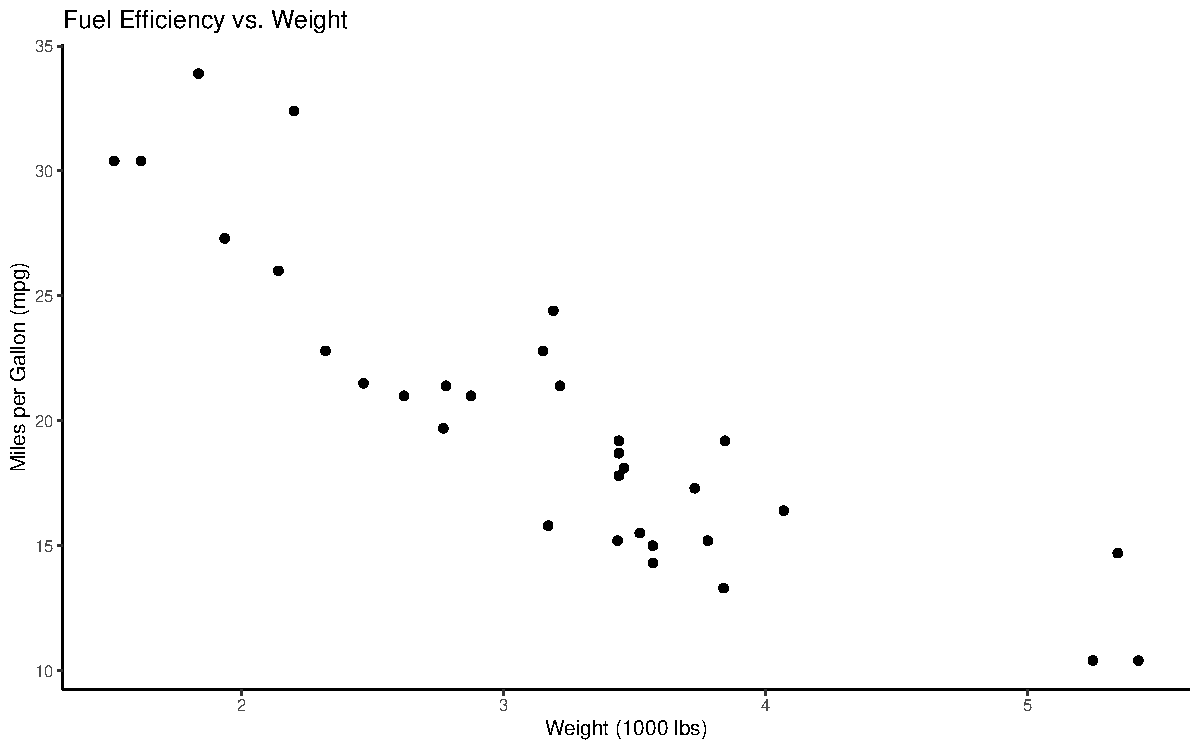
\includegraphics[width=\textwidth,height=0.5\textheight]{R-Regression_files/figure-beamer/unnamed-chunk-6-1.pdf}

}

\end{figure}

\begin{block}{Insights from Scatter Plot}
\protect\hypertarget{insights-from-scatter-plot}{}
\begin{itemize}
\tightlist
\item
  \textbf{Negative Correlation}: As weight increases, miles per gallon
  (mpg) generally decreases, indicating heavier cars are less
  fuel-efficient.
\end{itemize}

\normalsize
\end{block}
\end{block}
\end{frame}

\begin{frame}[fragile]{Box Plot: mpg by Number of Cylinders}
\protect\hypertarget{box-plot-mpg-by-number-of-cylinders}{}
\tiny

\begin{Shaded}
\begin{Highlighting}[]
\FunctionTok{ggplot}\NormalTok{(mtcars, }\FunctionTok{aes}\NormalTok{(}\AttributeTok{x =} \FunctionTok{factor}\NormalTok{(cyl), }\AttributeTok{y =}\NormalTok{ mpg)) }\SpecialCharTok{+}
  \FunctionTok{geom\_boxplot}\NormalTok{() }\SpecialCharTok{+}
  \FunctionTok{labs}\NormalTok{(}\AttributeTok{title =} \StringTok{"Fuel Efficiency by Number of Cylinders"}\NormalTok{,}
       \AttributeTok{x =} \StringTok{"Number of Cylinders"}\NormalTok{,}
       \AttributeTok{y =} \StringTok{"Miles per Gallon (mpg)"}\NormalTok{)}
\end{Highlighting}
\end{Shaded}

\begin{figure}

{\centering 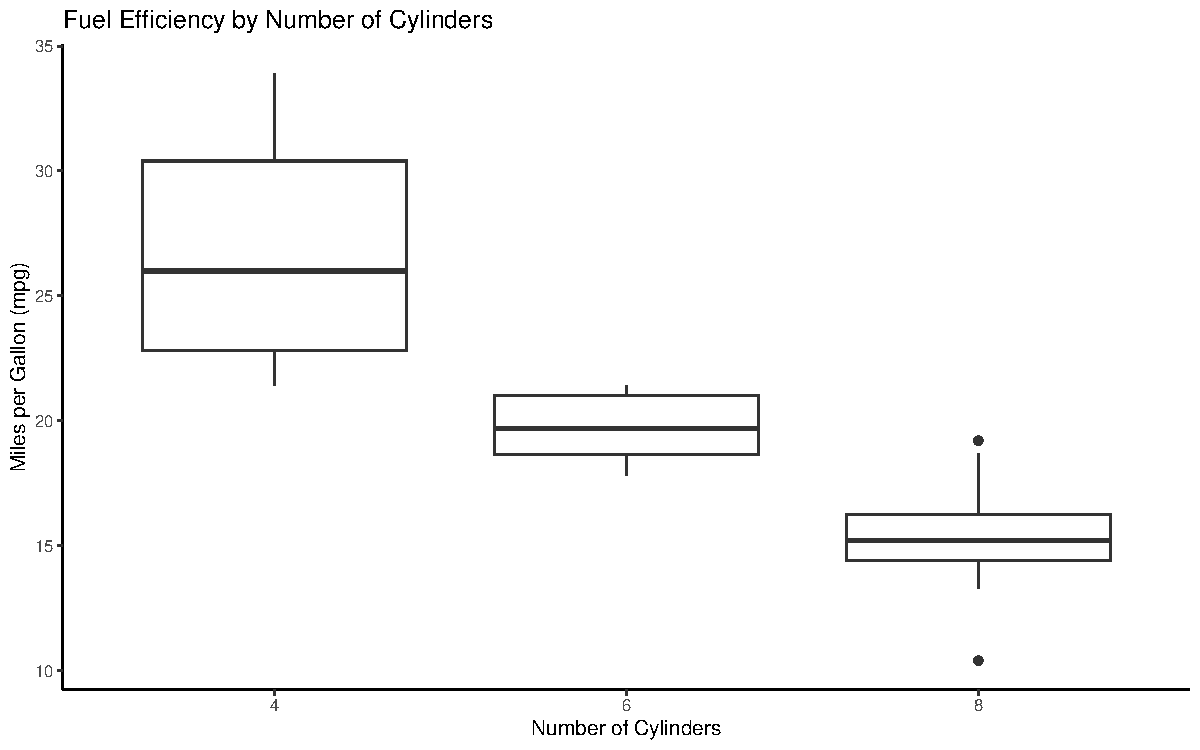
\includegraphics[width=\textwidth,height=0.5\textheight]{R-Regression_files/figure-beamer/unnamed-chunk-7-1.pdf}

}

\end{figure}

\begin{block}{Insights from Box Plot}
\protect\hypertarget{insights-from-box-plot}{}
\begin{itemize}
\tightlist
\item
  \textbf{Cylinders and mpg}: Cars with 4 cylinders tend to have the
  highest mpg, while cars with 8 cylinders have the lowest, indicating a
  trend where more cylinders correspond to less fuel efficiency.
  \normalsize
\end{itemize}
\end{block}
\end{frame}

\begin{frame}[fragile]{Correlation Analysis}
\protect\hypertarget{correlation-analysis}{}
\tiny

\begin{Shaded}
\begin{Highlighting}[]
\CommentTok{\# Correlation matrix}
\NormalTok{cor\_matrix }\OtherTok{\textless{}{-}} \FunctionTok{cor}\NormalTok{(mtcars)}
\FunctionTok{print}\NormalTok{(cor\_matrix)}
\CommentTok{\#\textgreater{}             mpg        cyl       disp         hp        drat         wt}
\CommentTok{\#\textgreater{} mpg   1.0000000 {-}0.8521620 {-}0.8475514 {-}0.7761684  0.68117191 {-}0.8676594}
\CommentTok{\#\textgreater{} cyl  {-}0.8521620  1.0000000  0.9020329  0.8324475 {-}0.69993811  0.7824958}
\CommentTok{\#\textgreater{} disp {-}0.8475514  0.9020329  1.0000000  0.7909486 {-}0.71021393  0.8879799}
\CommentTok{\#\textgreater{} hp   {-}0.7761684  0.8324475  0.7909486  1.0000000 {-}0.44875912  0.6587479}
\CommentTok{\#\textgreater{} drat  0.6811719 {-}0.6999381 {-}0.7102139 {-}0.4487591  1.00000000 {-}0.7124406}
\CommentTok{\#\textgreater{} wt   {-}0.8676594  0.7824958  0.8879799  0.6587479 {-}0.71244065  1.0000000}
\CommentTok{\#\textgreater{} qsec  0.4186840 {-}0.5912421 {-}0.4336979 {-}0.7082234  0.09120476 {-}0.1747159}
\CommentTok{\#\textgreater{} vs    0.6640389 {-}0.8108118 {-}0.7104159 {-}0.7230967  0.44027846 {-}0.5549157}
\CommentTok{\#\textgreater{} am    0.5998324 {-}0.5226070 {-}0.5912270 {-}0.2432043  0.71271113 {-}0.6924953}
\CommentTok{\#\textgreater{} gear  0.4802848 {-}0.4926866 {-}0.5555692 {-}0.1257043  0.69961013 {-}0.5832870}
\CommentTok{\#\textgreater{} carb {-}0.5509251  0.5269883  0.3949769  0.7498125 {-}0.09078980  0.4276059}
\CommentTok{\#\textgreater{}             qsec         vs          am       gear        carb}
\CommentTok{\#\textgreater{} mpg   0.41868403  0.6640389  0.59983243  0.4802848 {-}0.55092507}
\CommentTok{\#\textgreater{} cyl  {-}0.59124207 {-}0.8108118 {-}0.52260705 {-}0.4926866  0.52698829}
\CommentTok{\#\textgreater{} disp {-}0.43369788 {-}0.7104159 {-}0.59122704 {-}0.5555692  0.39497686}
\CommentTok{\#\textgreater{} hp   {-}0.70822339 {-}0.7230967 {-}0.24320426 {-}0.1257043  0.74981247}
\CommentTok{\#\textgreater{} drat  0.09120476  0.4402785  0.71271113  0.6996101 {-}0.09078980}
\CommentTok{\#\textgreater{} wt   {-}0.17471588 {-}0.5549157 {-}0.69249526 {-}0.5832870  0.42760594}
\CommentTok{\#\textgreater{} qsec  1.00000000  0.7445354 {-}0.22986086 {-}0.2126822 {-}0.65624923}
\CommentTok{\#\textgreater{} vs    0.74453544  1.0000000  0.16834512  0.2060233 {-}0.56960714}
\CommentTok{\#\textgreater{} am   {-}0.22986086  0.1683451  1.00000000  0.7940588  0.05753435}
\CommentTok{\#\textgreater{} gear {-}0.21268223  0.2060233  0.79405876  1.0000000  0.27407284}
\CommentTok{\#\textgreater{} carb {-}0.65624923 {-}0.5696071  0.05753435  0.2740728  1.00000000}
\end{Highlighting}
\end{Shaded}
\end{frame}

\begin{frame}[fragile]{Correlation Analysis}
\protect\hypertarget{correlation-analysis-1}{}
\tiny

\begin{Shaded}
\begin{Highlighting}[]
\CommentTok{\# Visualization of correlation matrix}
\FunctionTok{library}\NormalTok{(corrplot)}
\FunctionTok{corrplot}\NormalTok{(cor\_matrix,  }\AttributeTok{method =} \StringTok{\textquotesingle{}circle\textquotesingle{}}\NormalTok{, }\AttributeTok{type =} \StringTok{\textquotesingle{}upper\textquotesingle{}}\NormalTok{)}
\end{Highlighting}
\end{Shaded}

\begin{figure}

{\centering 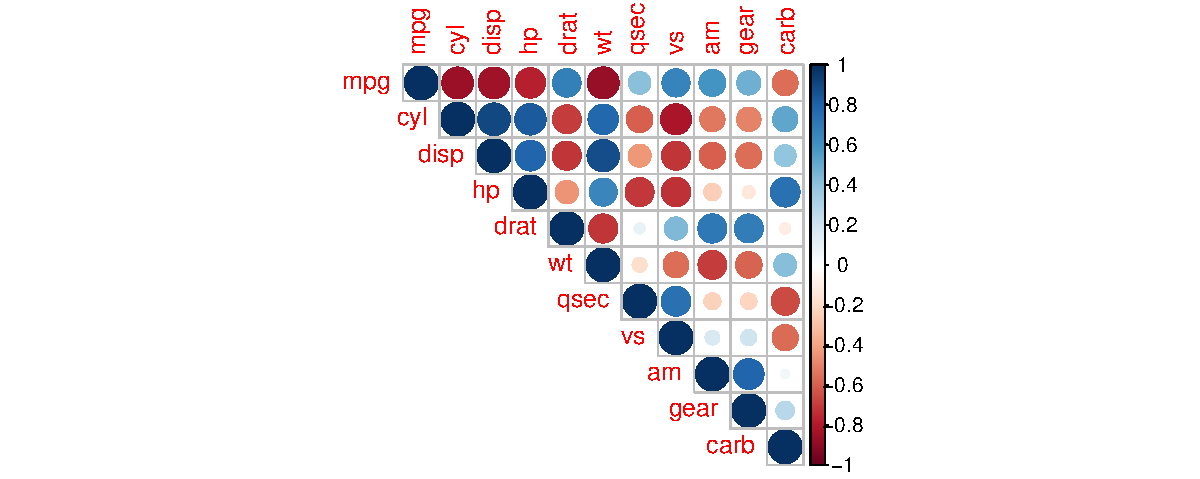
\includegraphics{R-Regression_files/figure-beamer/unnamed-chunk-9-1.pdf}

}

\end{figure}
\end{frame}

\begin{frame}{Correlation Analysis}
\protect\hypertarget{correlation-analysis-2}{}
\begin{block}{Insights from Correlation Matrix}
\protect\hypertarget{insights-from-correlation-matrix}{}
\begin{itemize}
\tightlist
\item
  \textbf{Strong Correlations}:

  \begin{itemize}
  \tightlist
  \item
    Positive correlation between \textbf{hp} (horsepower) and
    \textbf{mpg} (miles per gallon).
  \item
    Negative correlation between \textbf{wt} (weight) and \textbf{mpg}.
  \end{itemize}
\end{itemize}
\end{block}

\begin{block}{Conclusion}
\protect\hypertarget{conclusion}{}
\begin{itemize}
\tightlist
\item
  EDA highlights key relationships and patterns within the dataset,
  informing subsequent modeling approaches.
\end{itemize}

\normalsize
\end{block}
\end{frame}

\hypertarget{linear-regression}{%
\section{Linear Regression}\label{linear-regression}}

\begin{frame}[fragile]{Simple Linear Regression}
\protect\hypertarget{simple-linear-regression-1}{}
\begin{block}{Definition}
\protect\hypertarget{definition}{}
\begin{itemize}
\tightlist
\item
  Simple Linear Regression models the relationship between a dependent
  variable \(Y\) and one independent variable \(X\).
\item
  The goal is to predict or explain \(Y\) as a linear function of \(X\).
\end{itemize}
\end{block}

\begin{block}{Formula}
\protect\hypertarget{formula}{}
\begin{itemize}
\tightlist
\item
  The mathematical model for simple linear regression is:
  \(Y = \beta_0 + \beta_1 X + \epsilon\)

  \begin{itemize}
  \tightlist
  \item
    \(\beta_0\): Intercept (the value of \(Y\) when \(X = 0\))
  \item
    \(\beta_1\): Slope (the change in \(Y\) for a unit increase in
    \(X\))
  \item
    \(\epsilon\): Error term (accounts for the variability in \(Y\) that
    is not explained by \(X\))
  \end{itemize}
\end{itemize}
\end{block}

\begin{block}{Application}
\protect\hypertarget{application}{}
\begin{itemize}
\tightlist
\item
  Used for tasks such as predicting fuel efficiency based on vehicle
  weight (e.g., using \texttt{mpg} as \(Y\) and \texttt{wt} as \(X\)
  from the mtcars dataset).
\end{itemize}
\end{block}
\end{frame}

\begin{frame}[fragile]{Regression of mpg on wt}
\protect\hypertarget{regression-of-mpg-on-wt}{}
\begin{Shaded}
\begin{Highlighting}[]
\CommentTok{\# Simple Linear Regression in R}
\NormalTok{model }\OtherTok{\textless{}{-}} \FunctionTok{lm}\NormalTok{(mpg }\SpecialCharTok{\textasciitilde{}}\NormalTok{ wt, }\AttributeTok{data =}\NormalTok{ mtcars)}
\NormalTok{model}
\CommentTok{\#\textgreater{} }
\CommentTok{\#\textgreater{} Call:}
\CommentTok{\#\textgreater{} lm(formula = mpg \textasciitilde{} wt, data = mtcars)}
\CommentTok{\#\textgreater{} }
\CommentTok{\#\textgreater{} Coefficients:}
\CommentTok{\#\textgreater{} (Intercept)           wt  }
\CommentTok{\#\textgreater{}      37.285       {-}5.344}
\end{Highlighting}
\end{Shaded}

\normalsize
\end{frame}

\begin{frame}[fragile]{Regression of mpg on wt}
\protect\hypertarget{regression-of-mpg-on-wt-1}{}
\tiny

\begin{Shaded}
\begin{Highlighting}[]
\CommentTok{\# Simple Linear Regression in R}
\FunctionTok{summary}\NormalTok{(model)}
\CommentTok{\#\textgreater{} }
\CommentTok{\#\textgreater{} Call:}
\CommentTok{\#\textgreater{} lm(formula = mpg \textasciitilde{} wt, data = mtcars)}
\CommentTok{\#\textgreater{} }
\CommentTok{\#\textgreater{} Residuals:}
\CommentTok{\#\textgreater{}     Min      1Q  Median      3Q     Max }
\CommentTok{\#\textgreater{} {-}4.5432 {-}2.3647 {-}0.1252  1.4096  6.8727 }
\CommentTok{\#\textgreater{} }
\CommentTok{\#\textgreater{} Coefficients:}
\CommentTok{\#\textgreater{}             Estimate Std. Error t value Pr(\textgreater{}|t|)    }
\CommentTok{\#\textgreater{} (Intercept)  37.2851     1.8776  19.858  \textless{} 2e{-}16 ***}
\CommentTok{\#\textgreater{} wt           {-}5.3445     0.5591  {-}9.559 1.29e{-}10 ***}
\CommentTok{\#\textgreater{} {-}{-}{-}}
\CommentTok{\#\textgreater{} Signif. codes:  0 \textquotesingle{}***\textquotesingle{} 0.001 \textquotesingle{}**\textquotesingle{} 0.01 \textquotesingle{}*\textquotesingle{} 0.05 \textquotesingle{}.\textquotesingle{} 0.1 \textquotesingle{} \textquotesingle{} 1}
\CommentTok{\#\textgreater{} }
\CommentTok{\#\textgreater{} Residual standard error: 3.046 on 30 degrees of freedom}
\CommentTok{\#\textgreater{} Multiple R{-}squared:  0.7528, Adjusted R{-}squared:  0.7446 }
\CommentTok{\#\textgreater{} F{-}statistic: 91.38 on 1 and 30 DF,  p{-}value: 1.294e{-}10}
\end{Highlighting}
\end{Shaded}

\normalsize
\end{frame}

\begin{frame}[fragile]{Regression of mpg on wt}
\protect\hypertarget{regression-of-mpg-on-wt-2}{}
\tiny

\begin{Shaded}
\begin{Highlighting}[]
\CommentTok{\# Plot}
\FunctionTok{ggplot}\NormalTok{(mtcars, }\FunctionTok{aes}\NormalTok{(}\AttributeTok{x =}\NormalTok{ wt, }\AttributeTok{y =}\NormalTok{ mpg)) }\SpecialCharTok{+}
  \FunctionTok{geom\_point}\NormalTok{() }\SpecialCharTok{+}
  \FunctionTok{geom\_smooth}\NormalTok{(}\AttributeTok{method =} \StringTok{"lm"}\NormalTok{, }\AttributeTok{col =} \StringTok{"blue"}\NormalTok{) }\SpecialCharTok{+}
  \FunctionTok{labs}\NormalTok{(}\AttributeTok{title =} \StringTok{"Simple Linear Regression: mpg vs wt"}\NormalTok{,}
       \AttributeTok{x =} \StringTok{"Weight (1000 lbs)"}\NormalTok{,}
       \AttributeTok{y =} \StringTok{"Miles per Gallon (mpg)"}\NormalTok{)}
\end{Highlighting}
\end{Shaded}

\begin{figure}

{\centering 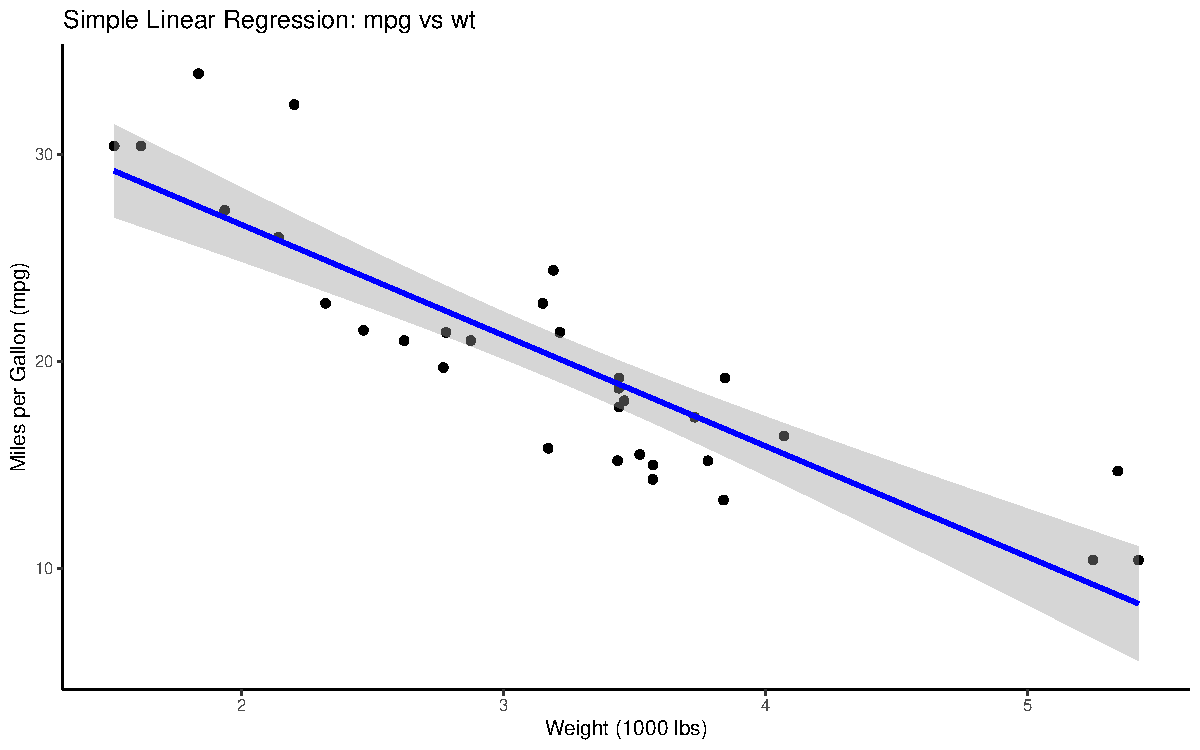
\includegraphics[width=\textwidth,height=0.5\textheight]{R-Regression_files/figure-beamer/unnamed-chunk-12-1.pdf}

}

\caption{Regression of mpg on wt}

\end{figure}

\normalsize

\begin{block}{Interpretation}
\protect\hypertarget{interpretation}{}
\begin{itemize}
\item
  **Slope (\(\beta_0\)) : Indicates the decrease in miles per gallon for
  every additional 1000 lbs of weight.
\item
  **Intercept (\(\beta_1\)): Predicts the mpg when weight is 0 (although
  not meaningful in this context).
\end{itemize}
\end{block}
\end{frame}

\begin{frame}[fragile]{Fitted values and residuals}
\protect\hypertarget{fitted-values-and-residuals}{}
\tiny

\begin{Shaded}
\begin{Highlighting}[]
\FunctionTok{library}\NormalTok{(broom)}
\FunctionTok{ggplot}\NormalTok{(}\FunctionTok{augment}\NormalTok{(model), }\FunctionTok{aes}\NormalTok{(wt, mpg)) }\SpecialCharTok{+}
  \FunctionTok{geom\_point}\NormalTok{() }\SpecialCharTok{+}
  \FunctionTok{stat\_smooth}\NormalTok{(}\AttributeTok{method =}\NormalTok{ lm, }\AttributeTok{se =} \ConstantTok{FALSE}\NormalTok{) }\SpecialCharTok{+}
  \FunctionTok{geom\_segment}\NormalTok{(}\FunctionTok{aes}\NormalTok{(}\AttributeTok{xend =}\NormalTok{ wt, }\AttributeTok{yend =}\NormalTok{ .fitted), }\AttributeTok{color =} \StringTok{"red"}\NormalTok{, }\AttributeTok{size =} \FloatTok{0.3}\NormalTok{)}
\end{Highlighting}
\end{Shaded}

\begin{figure}

{\centering 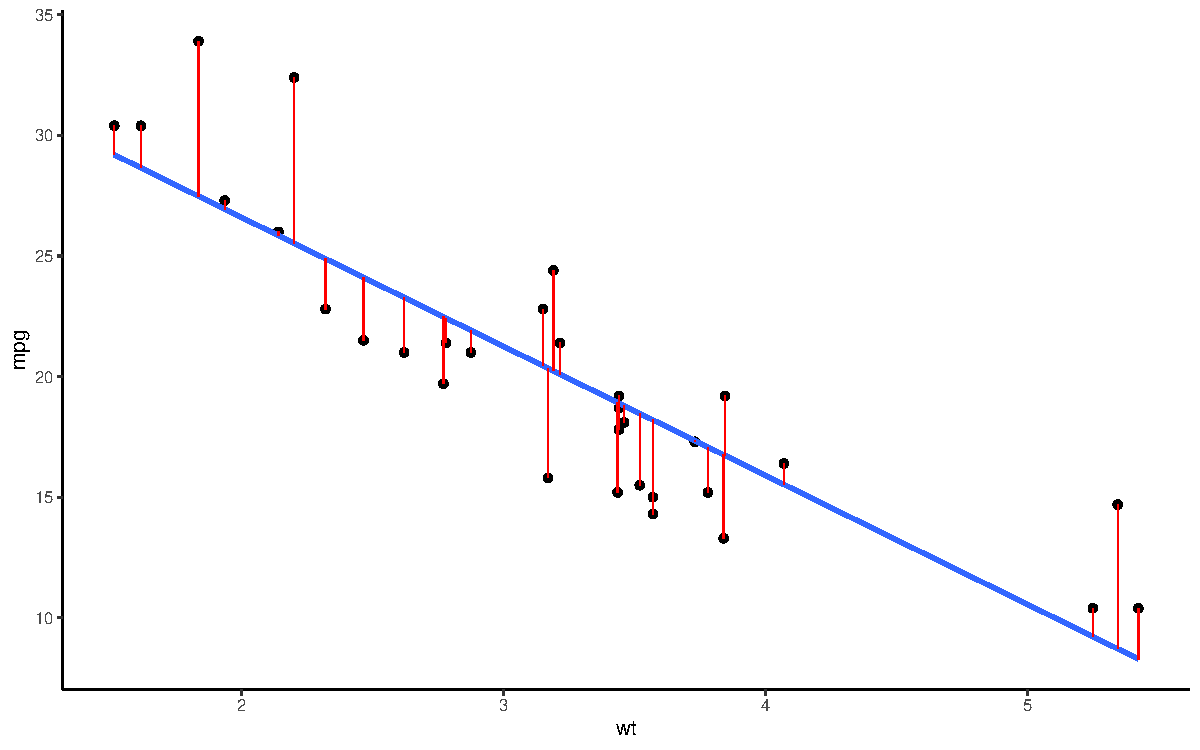
\includegraphics[width=\textwidth,height=0.5\textheight]{R-Regression_files/figure-beamer/unnamed-chunk-13-1.pdf}

}

\end{figure}
\end{frame}

\hypertarget{multiple-linear-regression-1}{%
\section{Multiple Linear
Regression}\label{multiple-linear-regression-1}}

\begin{frame}{Multiple Linear Regression with Two Factors}
\protect\hypertarget{multiple-linear-regression-with-two-factors}{}
\begin{block}{Definition}
\protect\hypertarget{definition-1}{}
\begin{itemize}
\tightlist
\item
  Multiple Linear Regression models the relationship between a dependent
  variable \(Y\) and two or more independent variables.
\end{itemize}
\end{block}

\begin{block}{Formula}
\protect\hypertarget{formula-1}{}
\begin{itemize}
\tightlist
\item
  The model for multiple linear regression with two independent
  variables \((X_1\) and \(X_2\)) is:
\end{itemize}

\(Y = \beta_0 + \beta_1 X_1 + \beta_2 X_2 + \epsilon\)

\begin{itemize}
\tightlist
\item
  \$ \beta\_1 \$: The effect of \(X_1\) on \(Y\), holding \(X_2\)
  constant.
\item
  \$ \beta\_2 \$: The effect of \(X_2\) on \(Y\), holding \(X_1\)
  constant.
\end{itemize}
\end{block}

\begin{block}{Application}
\protect\hypertarget{application-1}{}
\begin{itemize}
\tightlist
\item
  We can extend the mpg model by adding an additional factor, such as
  horsepower (hp) and weight (wt) as predictors of mpg.
\end{itemize}
\end{block}
\end{frame}

\begin{frame}[fragile]{Regression of mpg on wt and hp}
\protect\hypertarget{regression-of-mpg-on-wt-and-hp}{}
\begin{Shaded}
\begin{Highlighting}[]
\CommentTok{\# Multiple Linear Regression in R}
\NormalTok{model2 }\OtherTok{\textless{}{-}} \FunctionTok{lm}\NormalTok{(mpg }\SpecialCharTok{\textasciitilde{}}\NormalTok{ wt }\SpecialCharTok{+}\NormalTok{ hp, }\AttributeTok{data =}\NormalTok{ mtcars)}
\NormalTok{model2}
\CommentTok{\#\textgreater{} }
\CommentTok{\#\textgreater{} Call:}
\CommentTok{\#\textgreater{} lm(formula = mpg \textasciitilde{} wt + hp, data = mtcars)}
\CommentTok{\#\textgreater{} }
\CommentTok{\#\textgreater{} Coefficients:}
\CommentTok{\#\textgreater{} (Intercept)           wt           hp  }
\CommentTok{\#\textgreater{}    37.22727     {-}3.87783     {-}0.03177}
\end{Highlighting}
\end{Shaded}

\normalsize
\end{frame}

\begin{frame}[fragile]{Regression of mpg on wt and hp}
\protect\hypertarget{regression-of-mpg-on-wt-and-hp-1}{}
\tiny

\begin{Shaded}
\begin{Highlighting}[]
\CommentTok{\# Multiple Linear Regression in R}
\FunctionTok{summary}\NormalTok{(model2)}
\CommentTok{\#\textgreater{} }
\CommentTok{\#\textgreater{} Call:}
\CommentTok{\#\textgreater{} lm(formula = mpg \textasciitilde{} wt + hp, data = mtcars)}
\CommentTok{\#\textgreater{} }
\CommentTok{\#\textgreater{} Residuals:}
\CommentTok{\#\textgreater{}    Min     1Q Median     3Q    Max }
\CommentTok{\#\textgreater{} {-}3.941 {-}1.600 {-}0.182  1.050  5.854 }
\CommentTok{\#\textgreater{} }
\CommentTok{\#\textgreater{} Coefficients:}
\CommentTok{\#\textgreater{}             Estimate Std. Error t value Pr(\textgreater{}|t|)    }
\CommentTok{\#\textgreater{} (Intercept) 37.22727    1.59879  23.285  \textless{} 2e{-}16 ***}
\CommentTok{\#\textgreater{} wt          {-}3.87783    0.63273  {-}6.129 1.12e{-}06 ***}
\CommentTok{\#\textgreater{} hp          {-}0.03177    0.00903  {-}3.519  0.00145 ** }
\CommentTok{\#\textgreater{} {-}{-}{-}}
\CommentTok{\#\textgreater{} Signif. codes:  0 \textquotesingle{}***\textquotesingle{} 0.001 \textquotesingle{}**\textquotesingle{} 0.01 \textquotesingle{}*\textquotesingle{} 0.05 \textquotesingle{}.\textquotesingle{} 0.1 \textquotesingle{} \textquotesingle{} 1}
\CommentTok{\#\textgreater{} }
\CommentTok{\#\textgreater{} Residual standard error: 2.593 on 29 degrees of freedom}
\CommentTok{\#\textgreater{} Multiple R{-}squared:  0.8268, Adjusted R{-}squared:  0.8148 }
\CommentTok{\#\textgreater{} F{-}statistic: 69.21 on 2 and 29 DF,  p{-}value: 9.109e{-}12}
\end{Highlighting}
\end{Shaded}

\normalsize
\end{frame}

\begin{frame}{Regression of mpg on wt and hp}
\protect\hypertarget{regression-of-mpg-on-wt-and-hp-2}{}
\begin{block}{Interpretation}
\protect\hypertarget{interpretation-1}{}
\begin{itemize}
\tightlist
\item
  \textbf{Coefficients}:

  \begin{itemize}
  \item
    The coefficient for \textbf{wt} shows the change in mpg for every
    unit change in weight, holding horsepower constant.
  \item
    The coefficient for \textbf{hp} shows the change in mpg for every
    unit change in horsepower, holding weight constant.
  \end{itemize}
\item
  \textbf{Multiple R-squared}: Indicates how well the model explains the
  variability in mpg.
\end{itemize}
\end{block}
\end{frame}

\hypertarget{assumptions-of-linear-regression}{%
\section{Assumptions of Linear
Regression}\label{assumptions-of-linear-regression}}

\begin{frame}{Key Assumptions}
\protect\hypertarget{key-assumptions}{}
\begin{enumerate}
\tightlist
\item
  \textbf{Linearity}:

  \begin{itemize}
  \tightlist
  \item
    The relationship between the independent and dependent variables
    must be linear.
  \item
    This can be checked visually using scatter plots or residual plots.
  \end{itemize}
\item
  \textbf{Independence}:

  \begin{itemize}
  \tightlist
  \item
    Observations should be independent of each other.
  \item
    This is important for the validity of statistical inferences.
  \end{itemize}
\item
  \textbf{Homoscedasticity}:

  \begin{itemize}
  \tightlist
  \item
    The residuals (errors) should have constant variance across all
    levels of the independent variables.
  \item
    Can be checked using residual vs.~fitted value plots.
  \end{itemize}
\item
  \textbf{Normality of Residuals}:

  \begin{itemize}
  \tightlist
  \item
    The residuals should follow a normal distribution.
  \item
    This can be checked using a Q-Q plot or a histogram of residuals.
  \end{itemize}
\item
  \textbf{No Multicollinearity (for Multiple Regression)}:

  \begin{itemize}
  \tightlist
  \item
    Independent variables should not be highly correlated with each
    other.
  \item
    This can be checked using a correlation matrix or the Variance
    Inflation Factor (VIF).
  \end{itemize}
\end{enumerate}
\end{frame}

\begin{frame}[fragile]{Diagnostic Plots in R}
\protect\hypertarget{diagnostic-plots-in-r}{}
\begin{Shaded}
\begin{Highlighting}[]
\CommentTok{\# Diagnostic plots for model2}
\FunctionTok{par}\NormalTok{(}\AttributeTok{mfrow =} \FunctionTok{c}\NormalTok{(}\DecValTok{2}\NormalTok{, }\DecValTok{2}\NormalTok{), }\AttributeTok{mar =} \FunctionTok{c}\NormalTok{(}\DecValTok{4}\NormalTok{, }\DecValTok{4}\NormalTok{, }\DecValTok{2}\NormalTok{, }\DecValTok{1}\NormalTok{) )}
\FunctionTok{plot}\NormalTok{(model)}
\end{Highlighting}
\end{Shaded}
\end{frame}

\begin{frame}{Diagnostic Plots in R}
\protect\hypertarget{diagnostic-plots-in-r-1}{}
\begin{figure}

{\centering 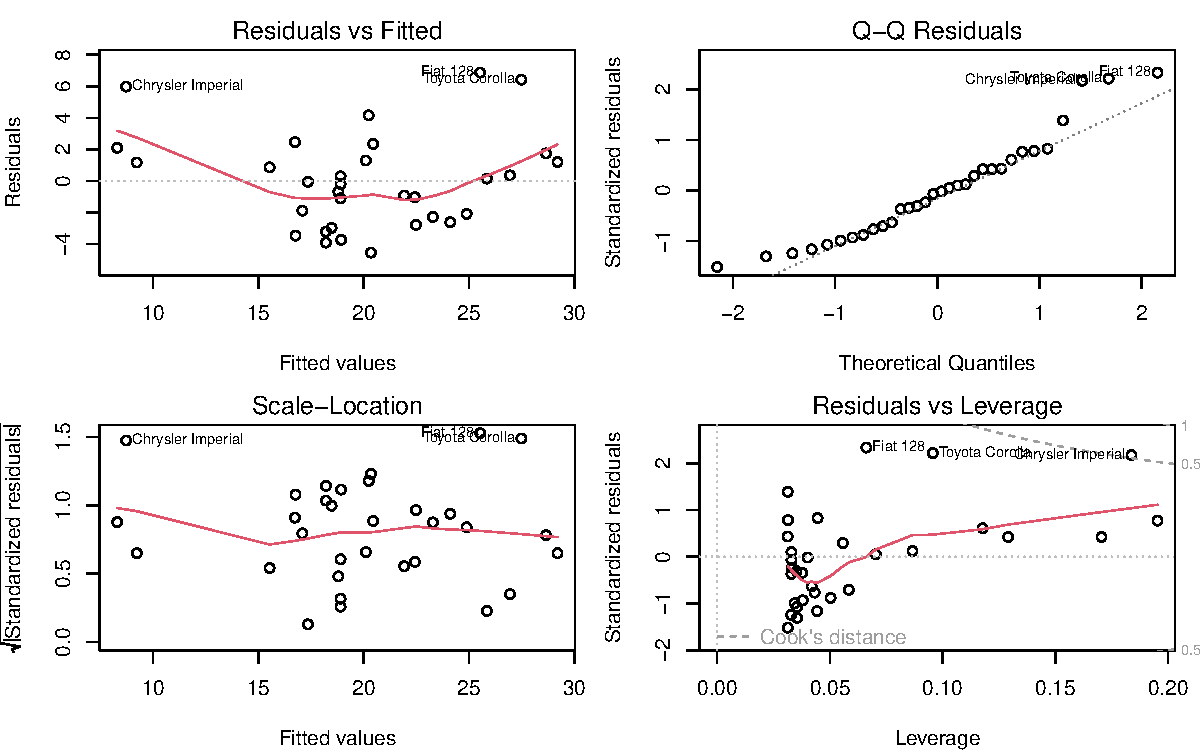
\includegraphics[width=\textwidth,height=0.6\textheight]{R-Regression_files/figure-beamer/unnamed-chunk-17-1.pdf}

}

\end{figure}
\end{frame}

\begin{frame}{Interpretation}
\protect\hypertarget{interpretation-2}{}
\begin{itemize}
\tightlist
\item
  Residuals vs Fitted: Checks for linearity and homoscedasticity.
\item
  Q-Q Plot: Checks for normality of residuals.
\item
  Scale-Location Plot: Checks for homoscedasticity.
\item
  Residuals vs Leverage: Identifies influential points.-
\end{itemize}
\end{frame}

\begin{frame}[fragile]{No Autocorrelation}
\protect\hypertarget{no-autocorrelation}{}
\begin{itemize}
\item
  \textbf{Definition}: The residuals should not be correlated with each
  other.
\item
  This assumption is crucial when working with time series or spatial
  data, where observations might be dependent over time or space.
\item
  \textbf{How to check}:

  \begin{itemize}
  \tightlist
  \item
    Plot residuals over time (for time series data).
  \item
    Use statistical tests like the \textbf{Durbin-Watson Test}.
  \end{itemize}
\end{itemize}

\tiny

\begin{Shaded}
\begin{Highlighting}[]
\CommentTok{\# Durbin{-}Watson test for autocorrelation}
\FunctionTok{library}\NormalTok{(lmtest)}
\FunctionTok{dwtest}\NormalTok{(model2)}
\CommentTok{\#\textgreater{} }
\CommentTok{\#\textgreater{}  Durbin{-}Watson test}
\CommentTok{\#\textgreater{} }
\CommentTok{\#\textgreater{} data:  model2}
\CommentTok{\#\textgreater{} DW = 1.3624, p{-}value = 0.02061}
\CommentTok{\#\textgreater{} alternative hypothesis: true autocorrelation is greater than 0}
\end{Highlighting}
\end{Shaded}

\normalsize
\end{frame}

\begin{frame}{Checking Linearity}
\protect\hypertarget{checking-linearity}{}
\begin{itemize}
\tightlist
\item
  The relationship between the independent variables and the dependent
  variable should be linear.
\end{itemize}

\begin{block}{How to check:}
\protect\hypertarget{how-to-check}{}
\begin{enumerate}
\tightlist
\item
  \textbf{Scatter Plot}: Plot each predictor against the response
  variable.
\item
  \textbf{Residuals vs Fitted Values}: Check for non-random patterns in
  the residuals.
\end{enumerate}
\end{block}
\end{frame}

\begin{frame}[fragile]{Checking Linearity}
\protect\hypertarget{checking-linearity-1}{}
\tiny

\begin{Shaded}
\begin{Highlighting}[]
\CommentTok{\# Checking Linearity using Residuals vs Fitted Plot}
\NormalTok{model }\OtherTok{\textless{}{-}} \FunctionTok{lm}\NormalTok{(mpg }\SpecialCharTok{\textasciitilde{}}\NormalTok{ wt }\SpecialCharTok{+}\NormalTok{ hp, }\AttributeTok{data =}\NormalTok{ mtcars)}
\FunctionTok{plot}\NormalTok{(model, }\AttributeTok{which =} \DecValTok{1}\NormalTok{)}
\end{Highlighting}
\end{Shaded}

\begin{figure}

{\centering 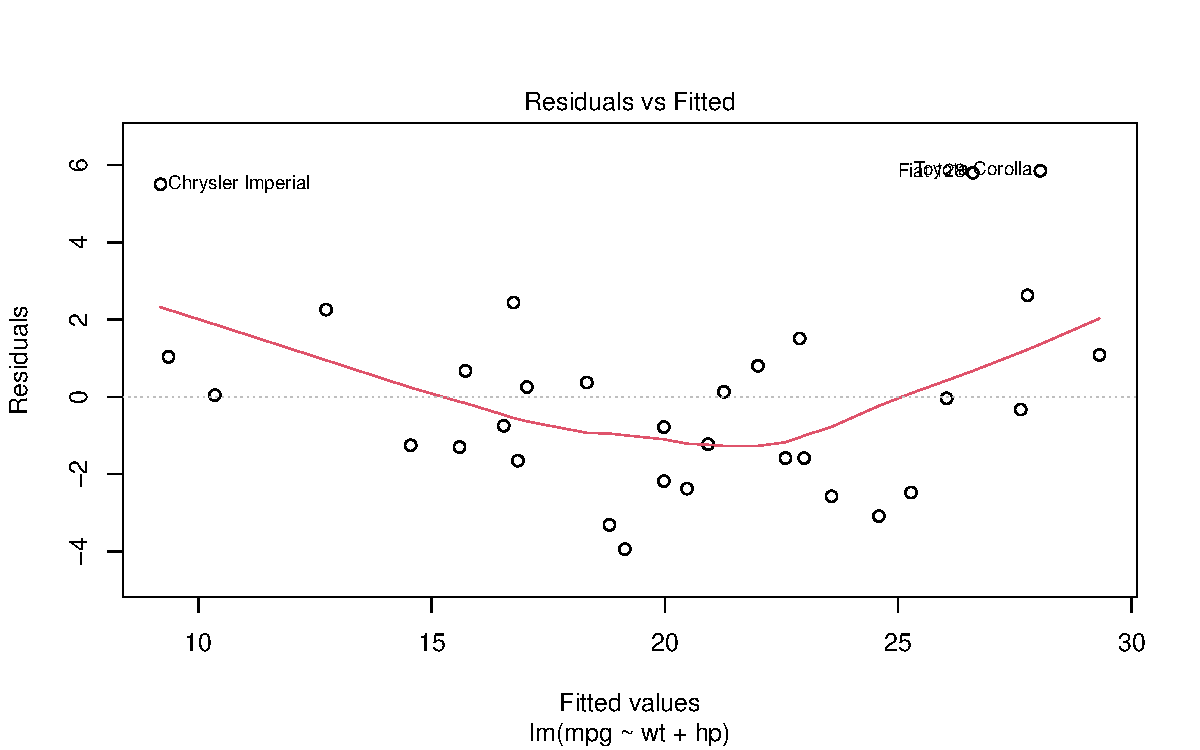
\includegraphics[width=\textwidth,height=0.5\textheight]{R-Regression_files/figure-beamer/unnamed-chunk-19-1.pdf}

}

\caption{Residuals vs Fitted Values Plot}

\end{figure}
\end{frame}

\begin{frame}{Checking Linearity}
\protect\hypertarget{checking-linearity-2}{}
\begin{block}{Interpretation}
\protect\hypertarget{interpretation-3}{}
\begin{itemize}
\tightlist
\item
  If the residuals are randomly scattered around zero with no clear
  pattern, the linearity assumption is likely satisfied.
\end{itemize}

\normalsize
\end{block}
\end{frame}

\begin{frame}[fragile]{Checking Independence}
\protect\hypertarget{checking-independence}{}
\begin{itemize}
\tightlist
\item
  Observations should be independent of one another. \tiny \#\#\# How to
  check:
\end{itemize}

\begin{enumerate}
\tightlist
\item
  \textbf{Durbin-Watson Test}: Used for detecting autocorrelation in
  residuals, particularly in time-series data.
\end{enumerate}

\begin{Shaded}
\begin{Highlighting}[]
\CommentTok{\# Checking Independence using Durbin{-}Watson Test}
\FunctionTok{library}\NormalTok{(lmtest)}
\FunctionTok{dwtest}\NormalTok{(model)}
\CommentTok{\#\textgreater{} }
\CommentTok{\#\textgreater{}  Durbin{-}Watson test}
\CommentTok{\#\textgreater{} }
\CommentTok{\#\textgreater{} data:  model}
\CommentTok{\#\textgreater{} DW = 1.3624, p{-}value = 0.02061}
\CommentTok{\#\textgreater{} alternative hypothesis: true autocorrelation is greater than 0}
\end{Highlighting}
\end{Shaded}

\begin{block}{Interpretation}
\protect\hypertarget{interpretation-4}{}
\begin{itemize}
\tightlist
\item
  A Durbin-Watson statistic close to 2 indicates no autocorrelation in
  the residuals.
\end{itemize}

\normalsize
\end{block}
\end{frame}

\begin{frame}{Checking Homoscedasticity}
\protect\hypertarget{checking-homoscedasticity}{}
\begin{itemize}
\tightlist
\item
  The residuals should have constant variance across all levels of the
  independent variables.
\end{itemize}

\begin{block}{How to check:}
\protect\hypertarget{how-to-check-1}{}
\begin{enumerate}
\tightlist
\item
  \textbf{Residuals vs Fitted Plot}: Look for a ``funnel'' shape,
  indicating heteroscedasticity.
\item
  \textbf{Breusch-Pagan Test}: A formal statistical test for
  heteroscedasticity.
\end{enumerate}
\end{block}
\end{frame}

\begin{frame}[fragile]{Checking Homoscedasticity}
\protect\hypertarget{checking-homoscedasticity-1}{}
\tiny

\begin{Shaded}
\begin{Highlighting}[]
\CommentTok{\# Checking Homoscedasticity using Residuals vs Fitted Plot}
\FunctionTok{plot}\NormalTok{(model, }\AttributeTok{which =} \DecValTok{3}\NormalTok{)}
\end{Highlighting}
\end{Shaded}

\begin{figure}

{\centering 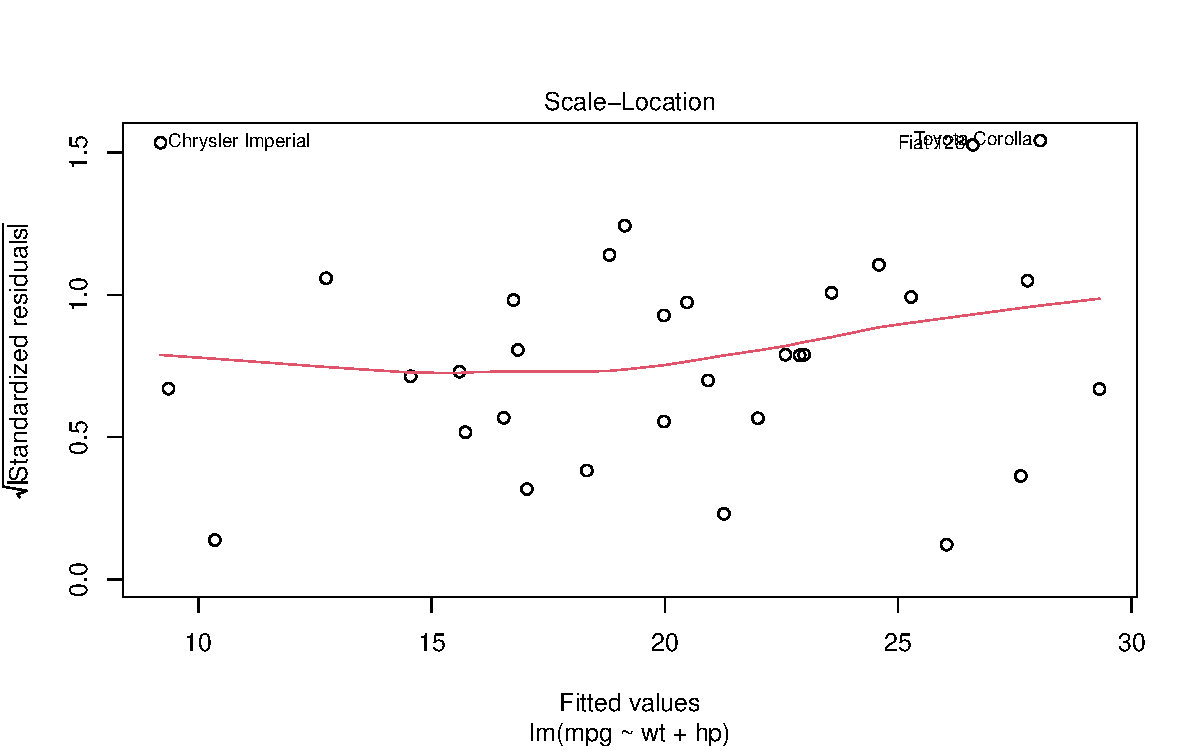
\includegraphics[width=\textwidth,height=0.5\textheight]{R-Regression_files/figure-beamer/unnamed-chunk-21-1.pdf}

}

\caption{Residuals vs Fitted Plot}

\end{figure}

\normalsize
\end{frame}

\begin{frame}[fragile]{Checking Homoscedasticity}
\protect\hypertarget{checking-homoscedasticity-2}{}
\begin{Shaded}
\begin{Highlighting}[]
\CommentTok{\# Breusch{-}Pagan test}
\FunctionTok{library}\NormalTok{(lmtest)}
\FunctionTok{bptest}\NormalTok{(model)}
\CommentTok{\#\textgreater{} }
\CommentTok{\#\textgreater{}  studentized Breusch{-}Pagan test}
\CommentTok{\#\textgreater{} }
\CommentTok{\#\textgreater{} data:  model}
\CommentTok{\#\textgreater{} BP = 0.88072, df = 2, p{-}value = 0.6438}
\end{Highlighting}
\end{Shaded}

\begin{block}{Interpretation}
\protect\hypertarget{interpretation-5}{}
\begin{itemize}
\tightlist
\item
  If the residuals fan out or show a pattern, the assumption of
  homoscedasticity may be violated.
\item
  The Breusch-Pagan test p-value should be greater than 0.05 to satisfy
  this assumption.
\end{itemize}

\normalsize
\end{block}
\end{frame}

\begin{frame}{Checking Normality of Residuals}
\protect\hypertarget{checking-normality-of-residuals}{}
\begin{itemize}
\tightlist
\item
  The residuals should follow a normal distribution.
\end{itemize}

\begin{block}{How to check:}
\protect\hypertarget{how-to-check-2}{}
\begin{enumerate}
\tightlist
\item
  \textbf{Q-Q Plot}: Visually assess the normality of residuals.
\item
  \textbf{Shapiro-Wilk Test}: A statistical test for normality.
\end{enumerate}
\end{block}
\end{frame}

\begin{frame}[fragile]{Checking Normality of Residuals}
\protect\hypertarget{checking-normality-of-residuals-1}{}
\tiny

\begin{Shaded}
\begin{Highlighting}[]
\CommentTok{\# Checking Normality using Q{-}Q Plot}
\FunctionTok{plot}\NormalTok{(model, }\AttributeTok{which =} \DecValTok{2}\NormalTok{)}
\end{Highlighting}
\end{Shaded}

\begin{figure}

{\centering 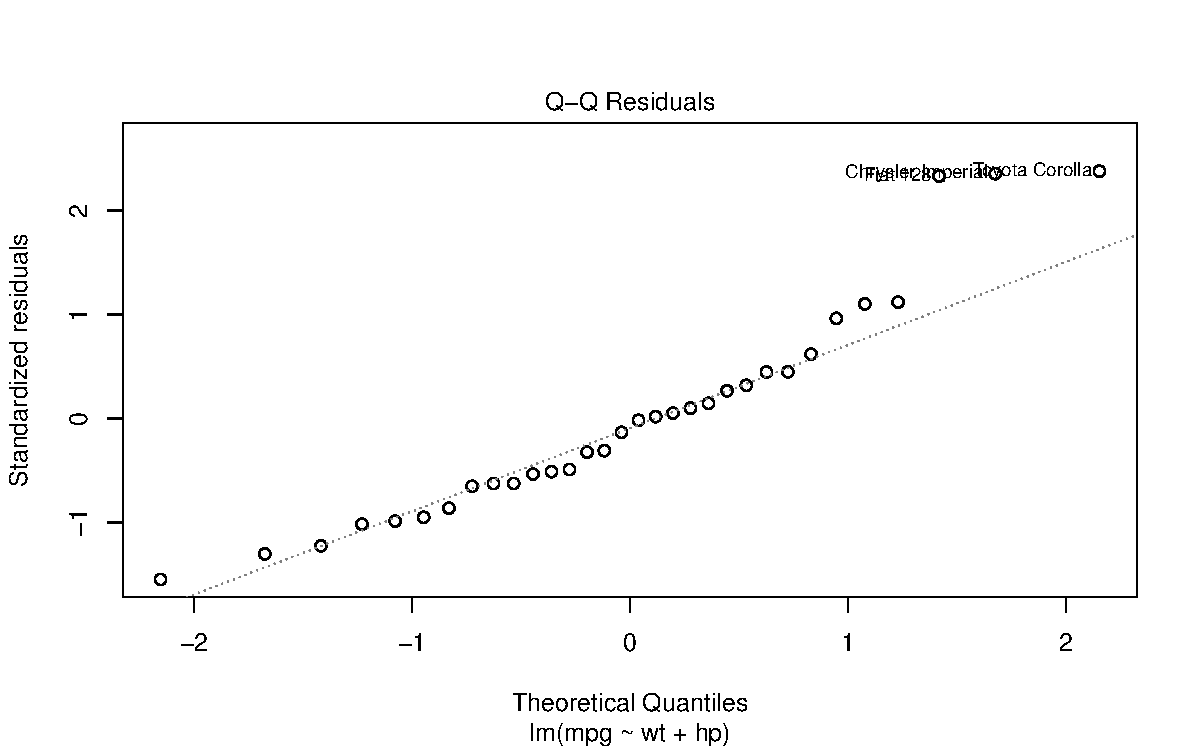
\includegraphics[width=\textwidth,height=0.5\textheight]{R-Regression_files/figure-beamer/unnamed-chunk-23-1.pdf}

}

\caption{Q-Q Plot}

\end{figure}
\end{frame}

\begin{frame}[fragile]{Checking Normality of Residuals}
\protect\hypertarget{checking-normality-of-residuals-2}{}
\begin{Shaded}
\begin{Highlighting}[]
\CommentTok{\# Shapiro{-}Wilk test}
\FunctionTok{shapiro.test}\NormalTok{(}\FunctionTok{residuals}\NormalTok{(model))}
\CommentTok{\#\textgreater{} }
\CommentTok{\#\textgreater{}  Shapiro{-}Wilk normality test}
\CommentTok{\#\textgreater{} }
\CommentTok{\#\textgreater{} data:  residuals(model)}
\CommentTok{\#\textgreater{} W = 0.92792, p{-}value = 0.03427}
\end{Highlighting}
\end{Shaded}

\begin{block}{Interpretation}
\protect\hypertarget{interpretation-6}{}
\begin{itemize}
\tightlist
\item
  If the points in the Q-Q plot roughly follow a straight line, the
  residuals are approximately normally distributed.
\item
  A p-value \textgreater{} 0.05 in the Shapiro-Wilk test suggests the
  residuals are normally distributed.
\end{itemize}
\end{block}
\end{frame}

\begin{frame}[fragile]{Checking for Multicollinearity}
\protect\hypertarget{checking-for-multicollinearity}{}
\begin{itemize}
\tightlist
\item
  Independent variables should not be highly correlated with each other.
\end{itemize}

\begin{block}{How to check:}
\protect\hypertarget{how-to-check-3}{}
\begin{enumerate}
\tightlist
\item
  \textbf{Variance Inflation Factor (VIF)}: Detects the presence of
  multicollinearity.
\item
  \textbf{Correlation Matrix}: Visually inspect correlations between
  variables.
\end{enumerate}

\begin{Shaded}
\begin{Highlighting}[]
\CommentTok{\# Checking Multicollinearity using VIF}
\FunctionTok{library}\NormalTok{(car)}
\FunctionTok{vif}\NormalTok{(model)}
\CommentTok{\#\textgreater{}       wt       hp }
\CommentTok{\#\textgreater{} 1.766625 1.766625}
\end{Highlighting}
\end{Shaded}
\end{block}
\end{frame}

\begin{frame}[fragile]{Checking for Multicollinearity}
\protect\hypertarget{checking-for-multicollinearity-1}{}
\begin{Shaded}
\begin{Highlighting}[]
\CommentTok{\# Correlation matrix of predictors}
\FunctionTok{cor}\NormalTok{(mtcars[, }\FunctionTok{c}\NormalTok{(}\StringTok{"wt"}\NormalTok{, }\StringTok{"hp"}\NormalTok{, }\StringTok{"mpg"}\NormalTok{)])}
\CommentTok{\#\textgreater{}             wt         hp        mpg}
\CommentTok{\#\textgreater{} wt   1.0000000  0.6587479 {-}0.8676594}
\CommentTok{\#\textgreater{} hp   0.6587479  1.0000000 {-}0.7761684}
\CommentTok{\#\textgreater{} mpg {-}0.8676594 {-}0.7761684  1.0000000}
\end{Highlighting}
\end{Shaded}

\begin{block}{Interpretation}
\protect\hypertarget{interpretation-7}{}
\begin{itemize}
\tightlist
\item
  VIF values greater than 2 indicate problematic multicollinearity.
\item
  High correlations between predictors in the correlation matrix suggest
  multicollinearity.
\end{itemize}
\end{block}
\end{frame}

\hypertarget{logistic-regression-1}{%
\section{Logistic Regression}\label{logistic-regression-1}}

\begin{frame}[fragile]{Logistic Regression}
\protect\hypertarget{logistic-regression-2}{}
\begin{itemize}
\tightlist
\item
  Logistic regression is used when the dependent variable is categorical
  (binary or dichotomous).
\item
  It models the probability that a given outcome occurs, based on one or
  more independent variables.
\end{itemize}

\begin{block}{Formula}
\protect\hypertarget{formula-2}{}
\begin{itemize}
\item
  The logistic regression model is:

  \[ \log\left(\frac{p}{1 - p}\right) = \beta_0 + \beta_1 X_1 + \beta_2 X_2 + \dots + \beta_n X_n \]

  \begin{itemize}
  \tightlist
  \item
    Where \texttt{p} is the probability of the outcome of interest.
  \end{itemize}
\end{itemize}
\end{block}

\begin{block}{Example Application}
\protect\hypertarget{example-application}{}
\begin{itemize}
\tightlist
\item
  We'll model whether a car has high mpg (above 20) based on weight
  (\texttt{wt}) and horsepower (\texttt{hp}).
\end{itemize}
\end{block}
\end{frame}

\begin{frame}[fragile]{Logistic Regression Example (mtcars)}
\protect\hypertarget{logistic-regression-example-mtcars}{}
\begin{block}{Binary Outcome: High vs.~Low mpg}
\protect\hypertarget{binary-outcome-high-vs.-low-mpg}{}
Logistic regression is used when the dependent variable is binary (e.g.,
0/1 or Yes/No).

Since mtcars doesn't contain a direct binary outcome variable, we can
create one for demonstration purposes, such as whether a car has high
vs.~low miles-per-gallon (mpg \textgreater{} 20 or not). \tiny

\begin{Shaded}
\begin{Highlighting}[]
\CommentTok{\# Create binary outcome for mpg}
\NormalTok{mtcars}\SpecialCharTok{$}\NormalTok{mpg\_high }\OtherTok{\textless{}{-}} \FunctionTok{ifelse}\NormalTok{(mtcars}\SpecialCharTok{$}\NormalTok{mpg }\SpecialCharTok{\textgreater{}} \DecValTok{20}\NormalTok{, }\DecValTok{1}\NormalTok{, }\DecValTok{0}\NormalTok{)}
\end{Highlighting}
\end{Shaded}

\begin{Shaded}
\begin{Highlighting}[]
\CommentTok{\# Logistic regression model}
\NormalTok{log\_model }\OtherTok{\textless{}{-}} \FunctionTok{glm}\NormalTok{(mpg\_high }\SpecialCharTok{\textasciitilde{}}\NormalTok{ wt }\SpecialCharTok{+}\NormalTok{ hp, }\AttributeTok{data =}\NormalTok{ mtcars, }\AttributeTok{family =}\NormalTok{ binomial)}
\NormalTok{log\_model}
\CommentTok{\#\textgreater{} }
\CommentTok{\#\textgreater{} Call:  glm(formula = mpg\_high \textasciitilde{} wt + hp, family = binomial, data = mtcars)}
\CommentTok{\#\textgreater{} }
\CommentTok{\#\textgreater{} Coefficients:}
\CommentTok{\#\textgreater{} (Intercept)           wt           hp  }
\CommentTok{\#\textgreater{}     894.228     {-}202.865       {-}2.021  }
\CommentTok{\#\textgreater{} }
\CommentTok{\#\textgreater{} Degrees of Freedom: 31 Total (i.e. Null);  29 Residual}
\CommentTok{\#\textgreater{} Null Deviance:       43.86 }
\CommentTok{\#\textgreater{} Residual Deviance: 1.116e{-}08     AIC: 6}
\end{Highlighting}
\end{Shaded}
\end{block}
\end{frame}

\begin{frame}[fragile]{Logistic Regression Example (mtcars)}
\protect\hypertarget{logistic-regression-example-mtcars-1}{}
\tiny

\begin{Shaded}
\begin{Highlighting}[]
\FunctionTok{summary}\NormalTok{(log\_model)}
\CommentTok{\#\textgreater{} }
\CommentTok{\#\textgreater{} Call:}
\CommentTok{\#\textgreater{} glm(formula = mpg\_high \textasciitilde{} wt + hp, family = binomial, data = mtcars)}
\CommentTok{\#\textgreater{} }
\CommentTok{\#\textgreater{} Coefficients:}
\CommentTok{\#\textgreater{}               Estimate Std. Error z value Pr(\textgreater{}|z|)}
\CommentTok{\#\textgreater{} (Intercept)    894.228 365884.162   0.002    0.998}
\CommentTok{\#\textgreater{} wt            {-}202.865  84688.218  {-}0.002    0.998}
\CommentTok{\#\textgreater{} hp              {-}2.021    858.062  {-}0.002    0.998}
\CommentTok{\#\textgreater{} }
\CommentTok{\#\textgreater{} (Dispersion parameter for binomial family taken to be 1)}
\CommentTok{\#\textgreater{} }
\CommentTok{\#\textgreater{}     Null deviance: 4.3860e+01  on 31  degrees of freedom}
\CommentTok{\#\textgreater{} Residual deviance: 1.1156e{-}08  on 29  degrees of freedom}
\CommentTok{\#\textgreater{} AIC: 6}
\CommentTok{\#\textgreater{} }
\CommentTok{\#\textgreater{} Number of Fisher Scoring iterations: 25}
\end{Highlighting}
\end{Shaded}

\begin{block}{Interpretation}
\protect\hypertarget{interpretation-8}{}
\begin{itemize}
\tightlist
\item
  Coefficients: The log-odds of high mpg decrease as weight or
  horsepower increase.
\item
  Odds Ratio: The exponentiated coefficients represent the odds of
  having high mpg given a one-unit increase in weight or horsepower.
\end{itemize}
\end{block}
\end{frame}

\begin{frame}{Key Assumptions of Logistic Regression}
\protect\hypertarget{key-assumptions-of-logistic-regression}{}
\begin{enumerate}
\tightlist
\item
  \textbf{Linearity of the Logit}

  \begin{itemize}
  \tightlist
  \item
    The relationship between the independent variables and the log-odds
    of the dependent variable should be linear.
  \end{itemize}
\item
  \textbf{Independence of Errors}

  \begin{itemize}
  \tightlist
  \item
    Observations should be independent of each other.
  \end{itemize}
\item
  \textbf{No Multicollinearity}

  \begin{itemize}
  \tightlist
  \item
    Independent variables should not be highly correlated with each
    other.
  \end{itemize}
\item
  \textbf{Adequate Sample Size}

  \begin{itemize}
  \tightlist
  \item
    A sufficient number of events for each predictor is necessary for
    stable estimates.
  \end{itemize}
\end{enumerate}

We'll explore how to check these assumptions and interpret the results.
\end{frame}

\begin{frame}[fragile]{Linearity of the Logit}
\protect\hypertarget{linearity-of-the-logit}{}
\begin{itemize}
\tightlist
\item
  The relationship between the log-odds of the outcome and each
  predictor should be linear.
\end{itemize}

\begin{block}{How to check:}
\protect\hypertarget{how-to-check-4}{}
\begin{enumerate}
\tightlist
\item
  \textbf{Box-Tidwell Test}: A statistical test to check linearity of
  the logit.
\end{enumerate}

\tiny

\begin{Shaded}
\begin{Highlighting}[]
\CommentTok{\# Checking Linearity of Logit using Box{-}Tidwell Test}
\NormalTok{mtcars}\SpecialCharTok{$}\NormalTok{log\_wt }\OtherTok{\textless{}{-}} \FunctionTok{log}\NormalTok{(mtcars}\SpecialCharTok{$}\NormalTok{wt)}
\NormalTok{log\_model\_test }\OtherTok{\textless{}{-}} \FunctionTok{glm}\NormalTok{(mpg\_high }\SpecialCharTok{\textasciitilde{}}\NormalTok{ wt }\SpecialCharTok{+} \FunctionTok{I}\NormalTok{(wt }\SpecialCharTok{*}\NormalTok{ log\_wt) }\SpecialCharTok{+}\NormalTok{ hp, }\AttributeTok{data =}\NormalTok{ mtcars, }\AttributeTok{family =}\NormalTok{ binomial)}
\FunctionTok{summary}\NormalTok{(log\_model\_test)}
\CommentTok{\#\textgreater{} }
\CommentTok{\#\textgreater{} Call:}
\CommentTok{\#\textgreater{} glm(formula = mpg\_high \textasciitilde{} wt + I(wt * log\_wt) + hp, family = binomial, }
\CommentTok{\#\textgreater{}     data = mtcars)}
\CommentTok{\#\textgreater{} }
\CommentTok{\#\textgreater{} Coefficients:}
\CommentTok{\#\textgreater{}                  Estimate Std. Error   z value Pr(\textgreater{}|z|)    }
\CommentTok{\#\textgreater{} (Intercept)     1.239e+16  1.959e+08  63272684   \textless{}2e{-}16 ***}
\CommentTok{\#\textgreater{} wt             {-}5.784e+15  1.360e+08 {-}42540630   \textless{}2e{-}16 ***}
\CommentTok{\#\textgreater{} I(wt * log\_wt)  2.173e+15  6.084e+07  35709419   \textless{}2e{-}16 ***}
\CommentTok{\#\textgreater{} hp             {-}2.302e+13  2.364e+05 {-}97357716   \textless{}2e{-}16 ***}
\CommentTok{\#\textgreater{} {-}{-}{-}}
\CommentTok{\#\textgreater{} Signif. codes:  0 \textquotesingle{}***\textquotesingle{} 0.001 \textquotesingle{}**\textquotesingle{} 0.01 \textquotesingle{}*\textquotesingle{} 0.05 \textquotesingle{}.\textquotesingle{} 0.1 \textquotesingle{} \textquotesingle{} 1}
\CommentTok{\#\textgreater{} }
\CommentTok{\#\textgreater{} (Dispersion parameter for binomial family taken to be 1)}
\CommentTok{\#\textgreater{} }
\CommentTok{\#\textgreater{}     Null deviance:  43.86  on 31  degrees of freedom}
\CommentTok{\#\textgreater{} Residual deviance: 288.35  on 28  degrees of freedom}
\CommentTok{\#\textgreater{} AIC: 296.35}
\CommentTok{\#\textgreater{} }
\CommentTok{\#\textgreater{} Number of Fisher Scoring iterations: 10}
\end{Highlighting}
\end{Shaded}

Interpretation - If the interaction term (\(wt \times log(wt)\)) is
significant, the linearity assumption is violated.
\end{block}
\end{frame}

\begin{frame}[fragile]{Independence of Errors}
\protect\hypertarget{independence-of-errors}{}
\begin{itemize}
\tightlist
\item
  Residuals (errors) should be independent across observations.
\end{itemize}

\begin{block}{How to check:}
\protect\hypertarget{how-to-check-5}{}
\begin{enumerate}
\tightlist
\item
  \textbf{Durbin-Watson Test}: Used to check for autocorrelation in
  residuals (as in linear regression).
\end{enumerate}

\begin{Shaded}
\begin{Highlighting}[]
\CommentTok{\# Checking independence of errors using Durbin{-}Watson Test}
\FunctionTok{dwtest}\NormalTok{(log\_model)}
\CommentTok{\#\textgreater{} }
\CommentTok{\#\textgreater{}  Durbin{-}Watson test}
\CommentTok{\#\textgreater{} }
\CommentTok{\#\textgreater{} data:  log\_model}
\CommentTok{\#\textgreater{} DW = 1.3853, p{-}value = 0.0244}
\CommentTok{\#\textgreater{} alternative hypothesis: true autocorrelation is greater than 0}
\end{Highlighting}
\end{Shaded}
\end{block}

\begin{block}{Interpretation}
\protect\hypertarget{interpretation-9}{}
\begin{itemize}
\tightlist
\item
  A Durbin-Watson statistic close to 2 indicates that the errors are
  independent.
\end{itemize}
\end{block}
\end{frame}

\begin{frame}[fragile]{No Multicollinearity}
\protect\hypertarget{no-multicollinearity}{}
\begin{itemize}
\tightlist
\item
  Independent variables should not be highly correlated.
\end{itemize}

\begin{block}{How to check:}
\protect\hypertarget{how-to-check-6}{}
\begin{enumerate}
\tightlist
\item
  \textbf{Variance Inflation Factor (VIF)}: Detects multicollinearity.
\item
  \textbf{Correlation Matrix}: Visualize correlations between
  predictors.
\end{enumerate}

\begin{Shaded}
\begin{Highlighting}[]
\CommentTok{\# Checking Multicollinearity using VIF}
\FunctionTok{vif}\NormalTok{(log\_model)}
\CommentTok{\#\textgreater{}       wt       hp }
\CommentTok{\#\textgreater{} 4.234545 4.234545}
\end{Highlighting}
\end{Shaded}
\end{block}
\end{frame}

\begin{frame}[fragile]{No Multicollinearity}
\protect\hypertarget{no-multicollinearity-1}{}
\begin{Shaded}
\begin{Highlighting}[]
\CommentTok{\# Correlation matrix for predictors}
\FunctionTok{cor}\NormalTok{(mtcars[, }\FunctionTok{c}\NormalTok{(}\StringTok{"wt"}\NormalTok{, }\StringTok{"hp"}\NormalTok{)])}
\CommentTok{\#\textgreater{}           wt        hp}
\CommentTok{\#\textgreater{} wt 1.0000000 0.6587479}
\CommentTok{\#\textgreater{} hp 0.6587479 1.0000000}
\end{Highlighting}
\end{Shaded}

\begin{block}{Interpretation}
\protect\hypertarget{interpretation-10}{}
\begin{itemize}
\tightlist
\item
  VIF values greater than 5 suggest problematic multicollinearity.
\item
  High correlations in the correlation matrix also indicate
  multicollinearity.
\end{itemize}
\end{block}
\end{frame}

\begin{frame}[fragile]{Adequate Sample Size}
\protect\hypertarget{adequate-sample-size}{}
\begin{itemize}
\tightlist
\item
  Logistic regression requires a sufficient number of events (positive
  cases) per predictor.
\end{itemize}

\begin{block}{How to check:}
\protect\hypertarget{how-to-check-7}{}
\begin{enumerate}
\tightlist
\item
  \textbf{Events per Variable (EPV)}: A rule of thumb is at least 10
  events (cases where the outcome is 1) per independent variable.
\end{enumerate}

\begin{Shaded}
\begin{Highlighting}[]
\CommentTok{\# Check how many events we have for the binary outcome}
\FunctionTok{table}\NormalTok{(mtcars}\SpecialCharTok{$}\NormalTok{mpg\_high)}
\CommentTok{\#\textgreater{} }
\CommentTok{\#\textgreater{}  0  1 }
\CommentTok{\#\textgreater{} 18 14}
\end{Highlighting}
\end{Shaded}
\end{block}

\begin{block}{Interpretation}
\protect\hypertarget{interpretation-11}{}
\begin{itemize}
\tightlist
\item
  Ensure that the number of events (cases where mpg\_high == 1) divided
  by the number of predictors is greater than 10.
\end{itemize}
\end{block}
\end{frame}

\begin{frame}{Model Diagnostics -- Residuals and Influential Points}
\protect\hypertarget{model-diagnostics-residuals-and-influential-points}{}
\begin{block}{Diagnostic Plots}
\protect\hypertarget{diagnostic-plots}{}
\begin{itemize}
\tightlist
\item
  Even though logistic regression doesn't assume homoscedasticity or
  normality of residuals, checking residuals for extreme values and
  influential points is still useful.
\end{itemize}
\end{block}

\begin{block}{How to check:}
\protect\hypertarget{how-to-check-8}{}
\begin{enumerate}
\tightlist
\item
  \textbf{Residuals vs Fitted Plot}: Look for extreme residuals.
\item
  \textbf{Cook's Distance}: Identify influential points.
\end{enumerate}
\end{block}
\end{frame}

\begin{frame}[fragile]{Model Diagnostics -- Residuals and Influential
Points}
\protect\hypertarget{model-diagnostics-residuals-and-influential-points-1}{}
\tiny

\begin{Shaded}
\begin{Highlighting}[]
\CommentTok{\# Residuals vs Fitted Plot for Logistic Regression}
\FunctionTok{plot}\NormalTok{(log\_model, }\AttributeTok{which =} \DecValTok{1}\NormalTok{)}
\end{Highlighting}
\end{Shaded}

\begin{figure}

{\centering 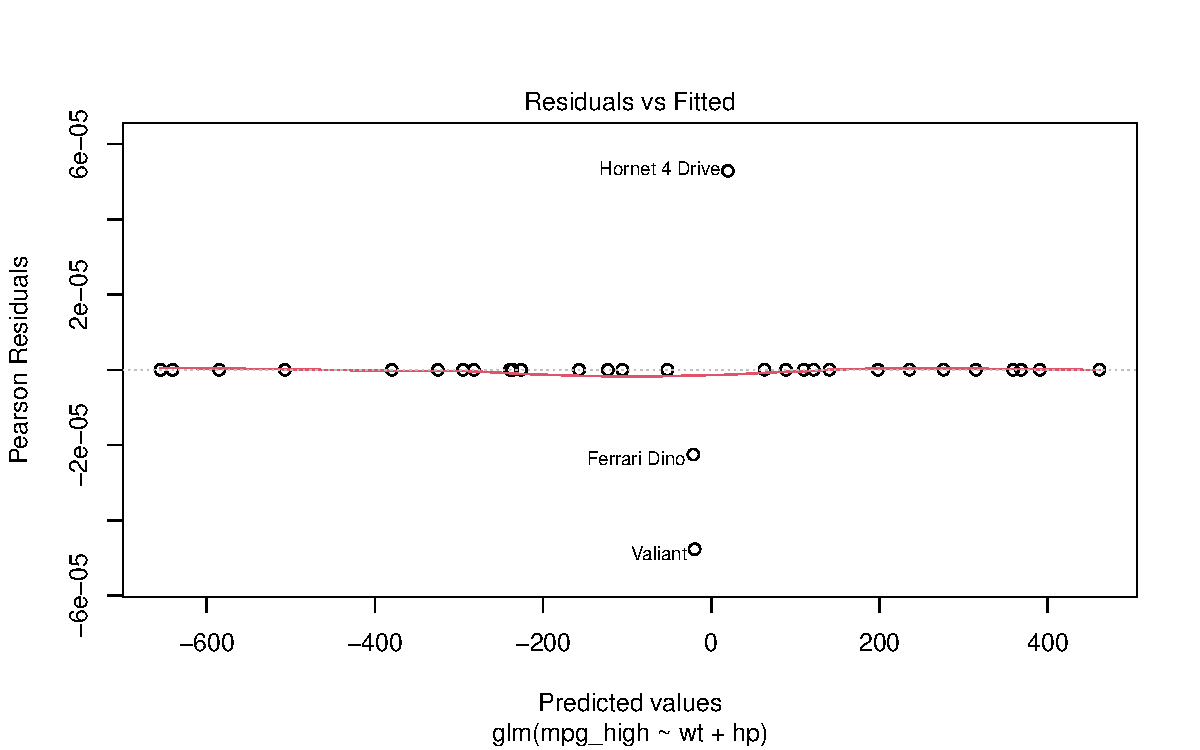
\includegraphics[width=\textwidth,height=0.5\textheight]{R-Regression_files/figure-beamer/unnamed-chunk-35-1.pdf}

}

\caption{Residuals vs Fitted Plot for Logistic Model}

\end{figure}
\end{frame}

\begin{frame}[fragile]{Model Diagnostics -- Residuals and Influential
Points}
\protect\hypertarget{model-diagnostics-residuals-and-influential-points-2}{}
\begin{block}{Cook's Distance to identify influential points}
\protect\hypertarget{cooks-distance-to-identify-influential-points}{}
\tiny

\begin{Shaded}
\begin{Highlighting}[]
\NormalTok{cooksd }\OtherTok{\textless{}{-}} \FunctionTok{cooks.distance}\NormalTok{(log\_model)}
\FunctionTok{plot}\NormalTok{(cooksd, }\AttributeTok{type =} \StringTok{"h"}\NormalTok{, }\AttributeTok{main =} \StringTok{"Cook\textquotesingle{}s Distance for Influential Points"}\NormalTok{)}
\end{Highlighting}
\end{Shaded}

\begin{figure}

{\centering 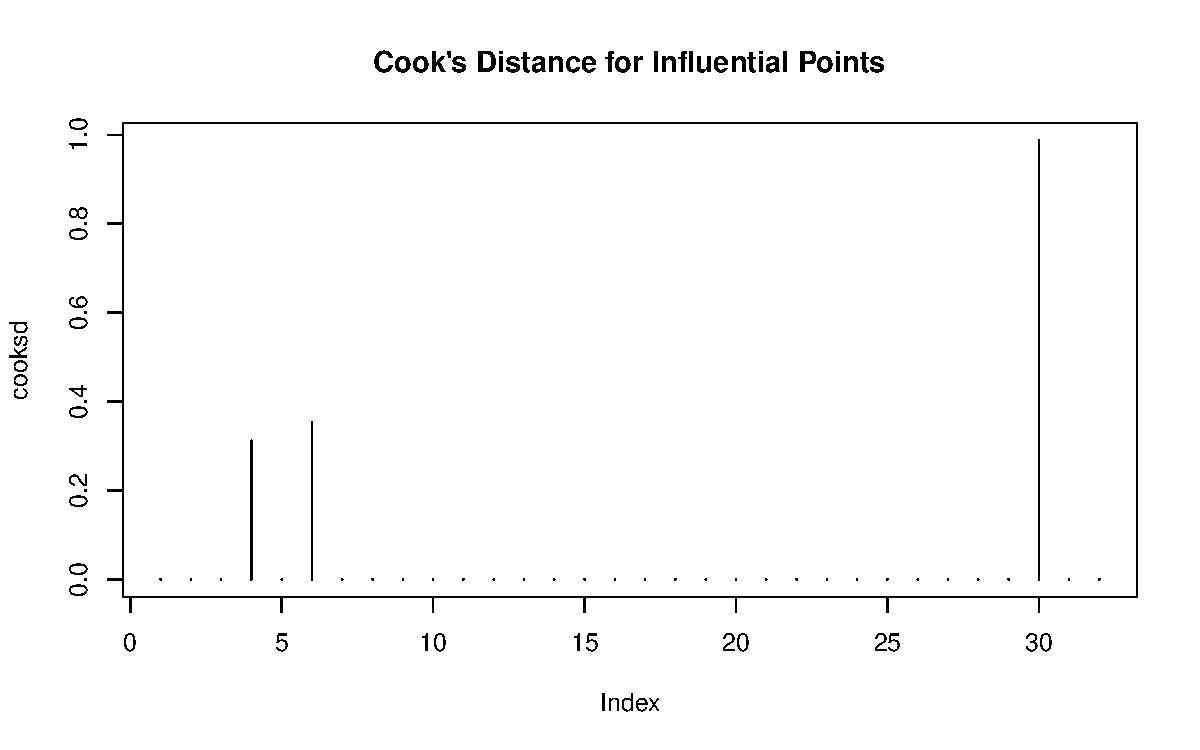
\includegraphics[width=\textwidth,height=0.5\textheight]{R-Regression_files/figure-beamer/unnamed-chunk-36-1.pdf}

}

\end{figure}

\tiny

\begin{block}{Interpretation}
\protect\hypertarget{interpretation-12}{}
\begin{itemize}
\tightlist
\item
  Residuals vs Fitted Plot: Look for residuals that significantly
  deviate from the main cluster.
\item
  Cook's Distance: Points with high Cook's Distance (\textgreater{} 1)
  could be influential.
\end{itemize}

Interpreting Odds Ratios \#\# Odds Ratios - Logistic regression
coefficients are in log-odds. To interpret them in more intuitive terms,
we can exponentiate the coefficients to get \textbf{odds ratios}.
\end{block}
\end{block}
\end{frame}

\begin{frame}[fragile]{Formula}
\protect\hypertarget{formula-3}{}
\(\text{Odds Ratio} = e^{\beta}\)

\begin{itemize}
\tightlist
\item
  This tells us the change in odds for a one-unit change in the
  predictor.
\end{itemize}

\begin{Shaded}
\begin{Highlighting}[]
\CommentTok{\# Calculate Odds Ratios}
\FunctionTok{exp}\NormalTok{(}\FunctionTok{coef}\NormalTok{(log\_model))}
\CommentTok{\#\textgreater{}  (Intercept)           wt           hp }
\CommentTok{\#\textgreater{}          Inf 7.884361e{-}89 1.325092e{-}01}
\end{Highlighting}
\end{Shaded}

\begin{block}{Interpretation}
\protect\hypertarget{interpretation-13}{}
\begin{itemize}
\tightlist
\item
  For each unit increase in weight (wt), the odds of having high mpg
  decrease by the calculated odds ratio.
\item
  For each unit increase in horsepower (hp), the odds of having high mpg
  also decrease by the calculated odds ratio.
\end{itemize}
\end{block}
\end{frame}

\begin{frame}{Thank You!}
\protect\hypertarget{thank-you}{}
\begin{itemize}
\tightlist
\item
  Thank you for your attention!
\item
  Feel free to reach out with any questions.
\end{itemize}

\begin{block}{Contact:}
\protect\hypertarget{contact}{}
\begin{itemize}
\tightlist
\item
  \textbf{Email}: mahesh.divakaran01@gmail.com
\item
  \textbf{LinkedIn}:
  \href{https://www.linkedin.com/in/imaheshdivakaran}{linkedin.com/in/imaheshdivakaran}
\end{itemize}
\end{block}
\end{frame}



\end{document}
